\documentclass[12pt, oneside,a4paper]{article}
\usepackage{ctex}
\usepackage{geometry}
\usepackage{indentfirst}               		
\usepackage{listings}
\usepackage{color}
\usepackage{textcomp}
\definecolor{dkgreen}{rgb}{0,0.6,0}
\definecolor{gray}{rgb}{0.5,0.5,0.5}
\definecolor{mauve}{rgb}{0.58,0,0.82}
\usepackage{amssymb,amsmath}
\usepackage[noend]{algpseudocode}
\usepackage{algorithmicx,algorithm}
\usepackage[font=small,labelfont={bf,sf},tableposition=top]{caption}
\usepackage{graphicx}
\usepackage{multirow}
\usepackage{float}
\usepackage{fancyhdr}
\lstset{frame=tb,
  language=Java,
  aboveskip=3mm,
  belowskip=3mm,
  showstringspaces=false,
  columns=flexible,
  basicstyle={\small\ttfamily},
  numbers=none,
  numberstyle=\tiny\color{gray},
  keywordstyle=\color{blue},
  commentstyle=\color{dkgreen},
  stringstyle=\color{mauve},
  breaklines=true,
  breakatwhitespace=true,
  tabsize=3
}
\geometry{a4paper,left=2cm,right=2cm,top=3cm,bottom=3cm}

\pagestyle{fancy}
\lhead{数据库引论 Project \# 1}
\rhead{胡天晓, 张昊晗, 刘婧源}

\newcommand{\HRule}{\rule{\linewidth}{0.5mm}}
\begin{document}

\begin{titlepage}
\begin{center}
% Upper part of the page
\textsc{\LARGE 复旦大学}\\[1.5cm]
\textsc{\Large 数据库引论}\\[0.5cm]
% Title
\HRule \\[0.4cm]
{ \huge \bfseries Project 1: Glutton}\\[0.4cm]
\HRule \\[1.5cm]

\includegraphics[width=2in]{logo.jpg}\\[1cm]
% Author
\begin{minipage}{0.4\textwidth}
\begin{flushleft} \large
\begin{center}
\emph{作者:}\\
胡天晓\\
张昊晗\\
刘婧源
\end{center}
\end{flushleft}
\end{minipage}
\vfill
% Bottom of the page
{\large \today}
\end{center}
\end{titlepage}

  \makeatletter
    \renewcommand{\thefigure}{\ifnum \c@section>\z@ \thesection-\fi \@arabic\c@figure}
    \renewcommand{\thetable}{\ifnum \c@section>\z@ \thesection-\fi \@arabic\c@table}
  \makeatother

%\par\setlength{\parindent}{1em}\normalsize
\section{项目简介}
 \begin{itemize}
  \item 项目背景
  \paragraph {Glutton数据库项目} 是为复旦大学(张江校区)的吃货们设计的外卖网页应用平台,以python链接SQL语言,web为前端,界面友好。使用者分为商家和用户,支持商家查询、创建、更改、删除菜品,用户查询商家、菜品,创建、更改、删除、评价订单等操作。
  \item 依赖库|组织架构
   flask/bootstrap/sqlite
  \item 项目文件树
  \item 运行方法
  \item flask简介
  \item bootstrap简介
  \item sqlite简介
  \item 用户密码md5加密
  \item 其他
 \end{itemize}

\section{项目细节}

 \subsection{针对用户的功能}
我们的web app面向张江地区的人民,可以随意选择喜欢的商家和菜品。主界面的最上方是导航栏——左侧有四个按钮:可以选择以用户或商家身份使用这个应用;在登录后,还可以查看自己的主页和订单。右侧和中部同为登录和注册按钮。最下方包含了作者、版权信息等。
 \begin{figure}[H]
   \centering
     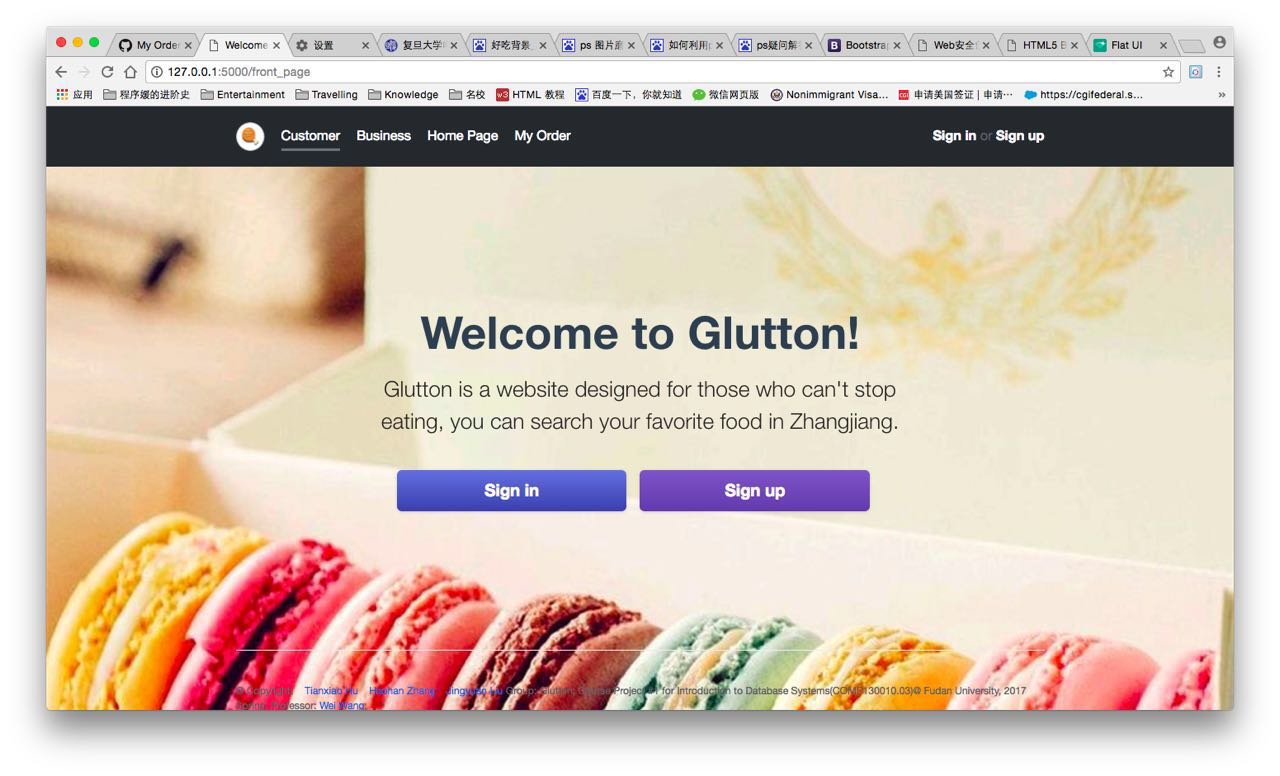
\includegraphics[width=6.00in]{cu-front.jpg}
     \caption{\small{主页面}}\label{fig:dummy}
  \end{figure}
  \begin{itemize}
  \item 注册/登录\\
  点击sign up按钮我们进入注册页面,输入用户名,手机号,密码来注册。手机号必须是唯一的,如果有重复,系统会提示这个手机号已经被注册,请直接登录。\\
  点击sign in按钮我们进入登录页面,用手机号和密码登录。如果密码输入错误,系统会提示密码或用户名错误。
  \begin{figure}[H]
   \begin{minipage}[t]{0.5\linewidth}
    \centering
     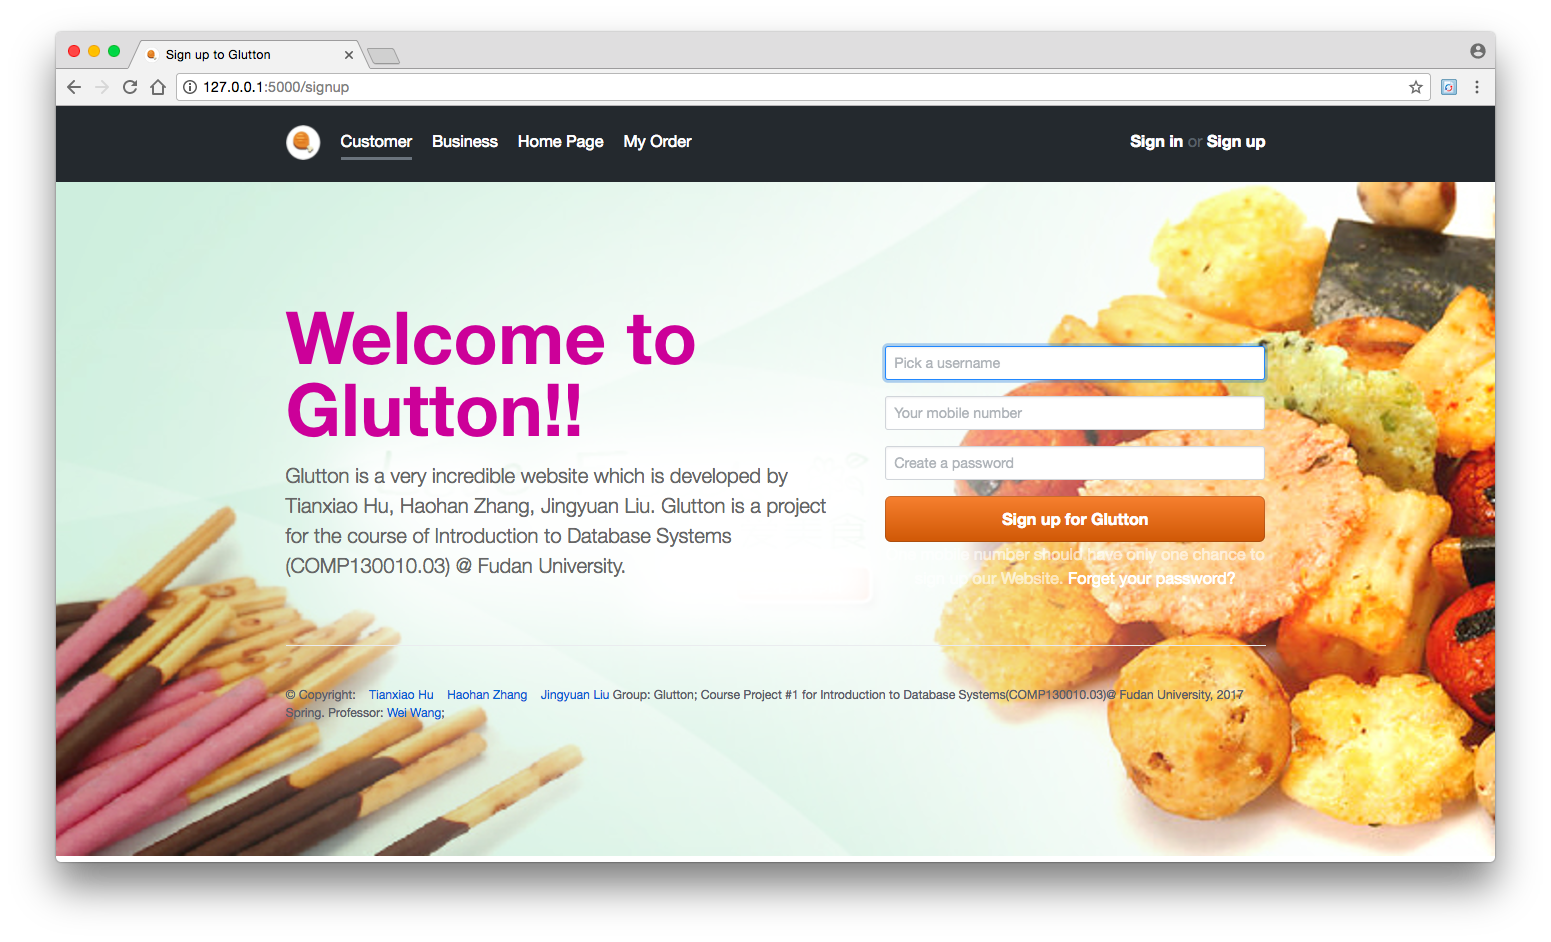
\includegraphics[width=3.2in]{cu-signup.jpg}
     \caption{\small{用户注册}}\label{fig:dummy}
   \end{minipage}
   \begin{minipage}[t]{0.5\linewidth}
    \centering
     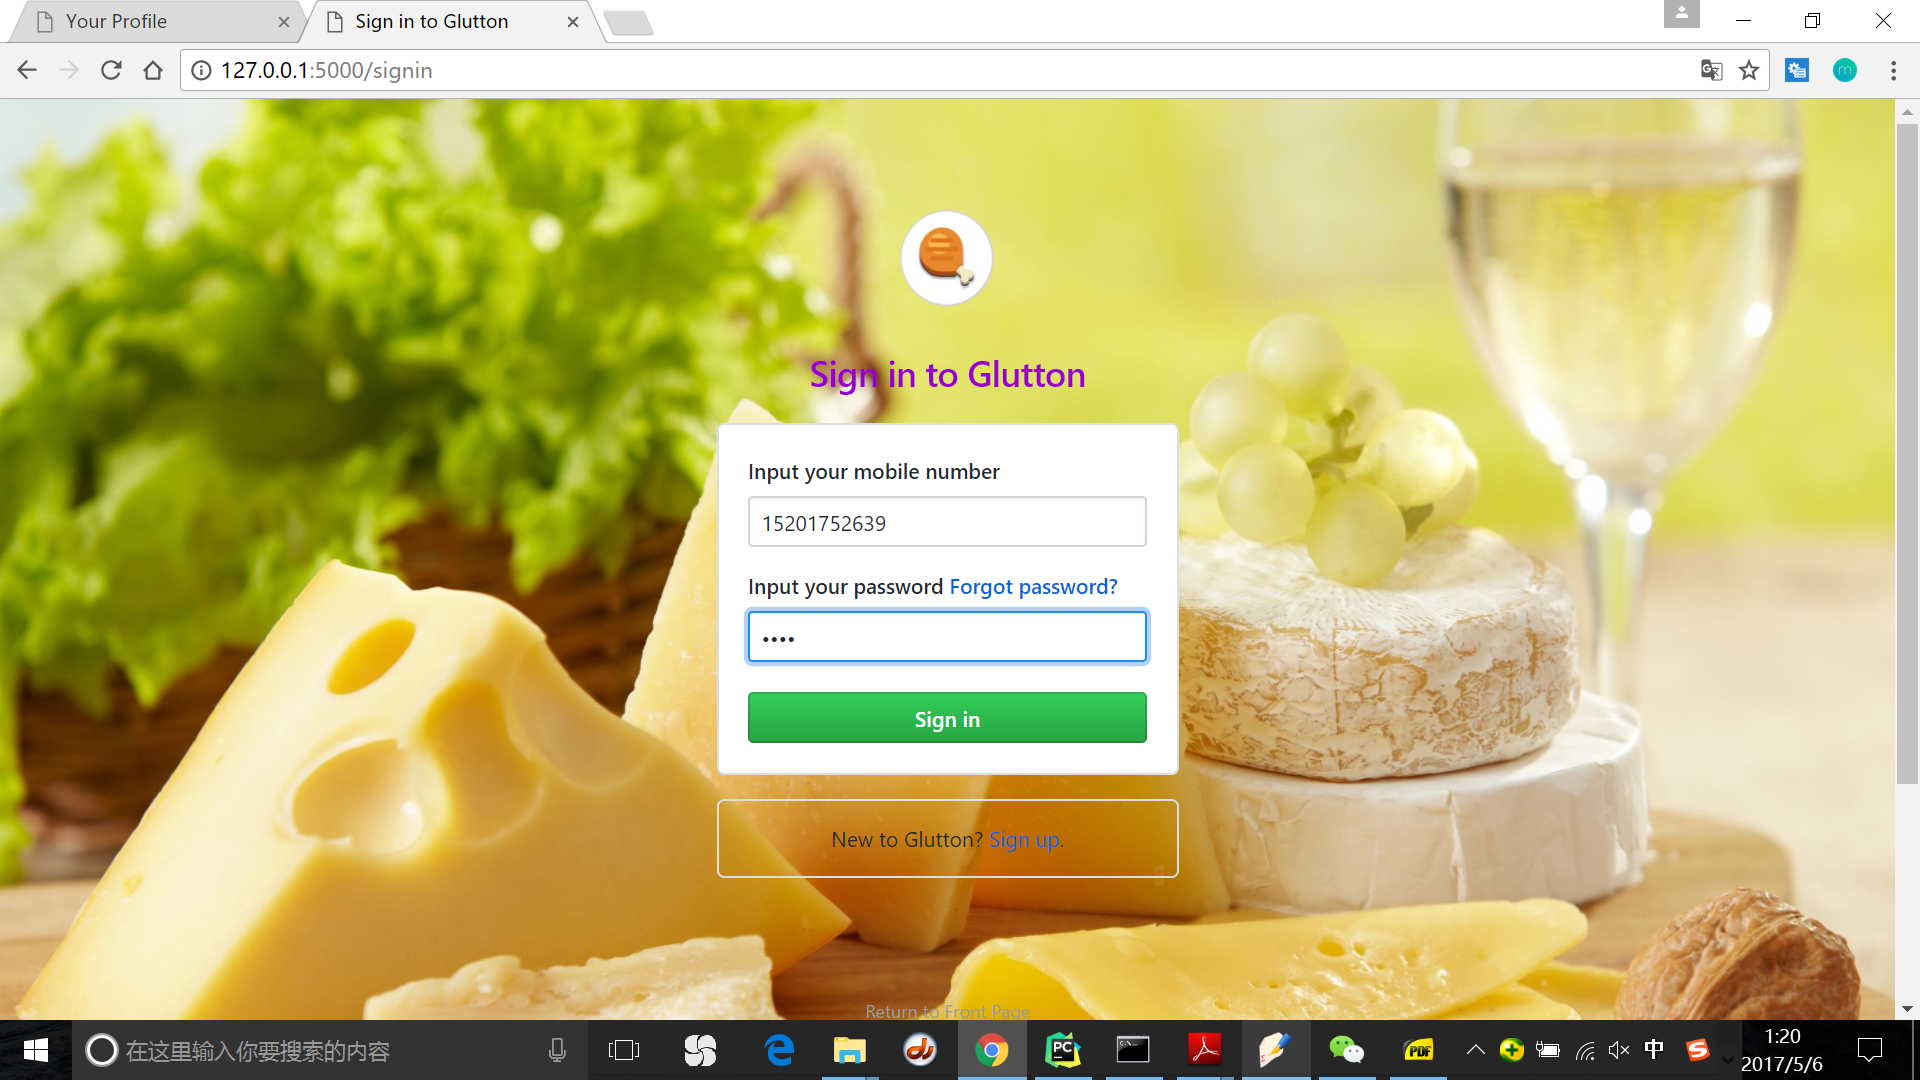
\includegraphics[width=3.2in]{cu-signin.jpg}
      \caption{\small{用户登录}}\label{fig:dummy}
   \end{minipage}
   \end{figure}
  \item 更改信息/头像\\
  登录成功后,我们进入到用户的主页。主页的最上方是导航栏,左侧三个按钮可以选择主页,个人信息,订单。右侧有搜索栏和退出登录按钮。
  左侧图片点击可以更改个人口味偏好,下方显示用户名和手机号,以及编辑个人信息按钮。中间同样有搜索栏,下方按食物分类配备了多种类型,如果汁奶茶、炸鸡汉堡等的食物分区,代表性商家可以直接鼠标点击进入。
  \begin{figure}[H]
   \centering
     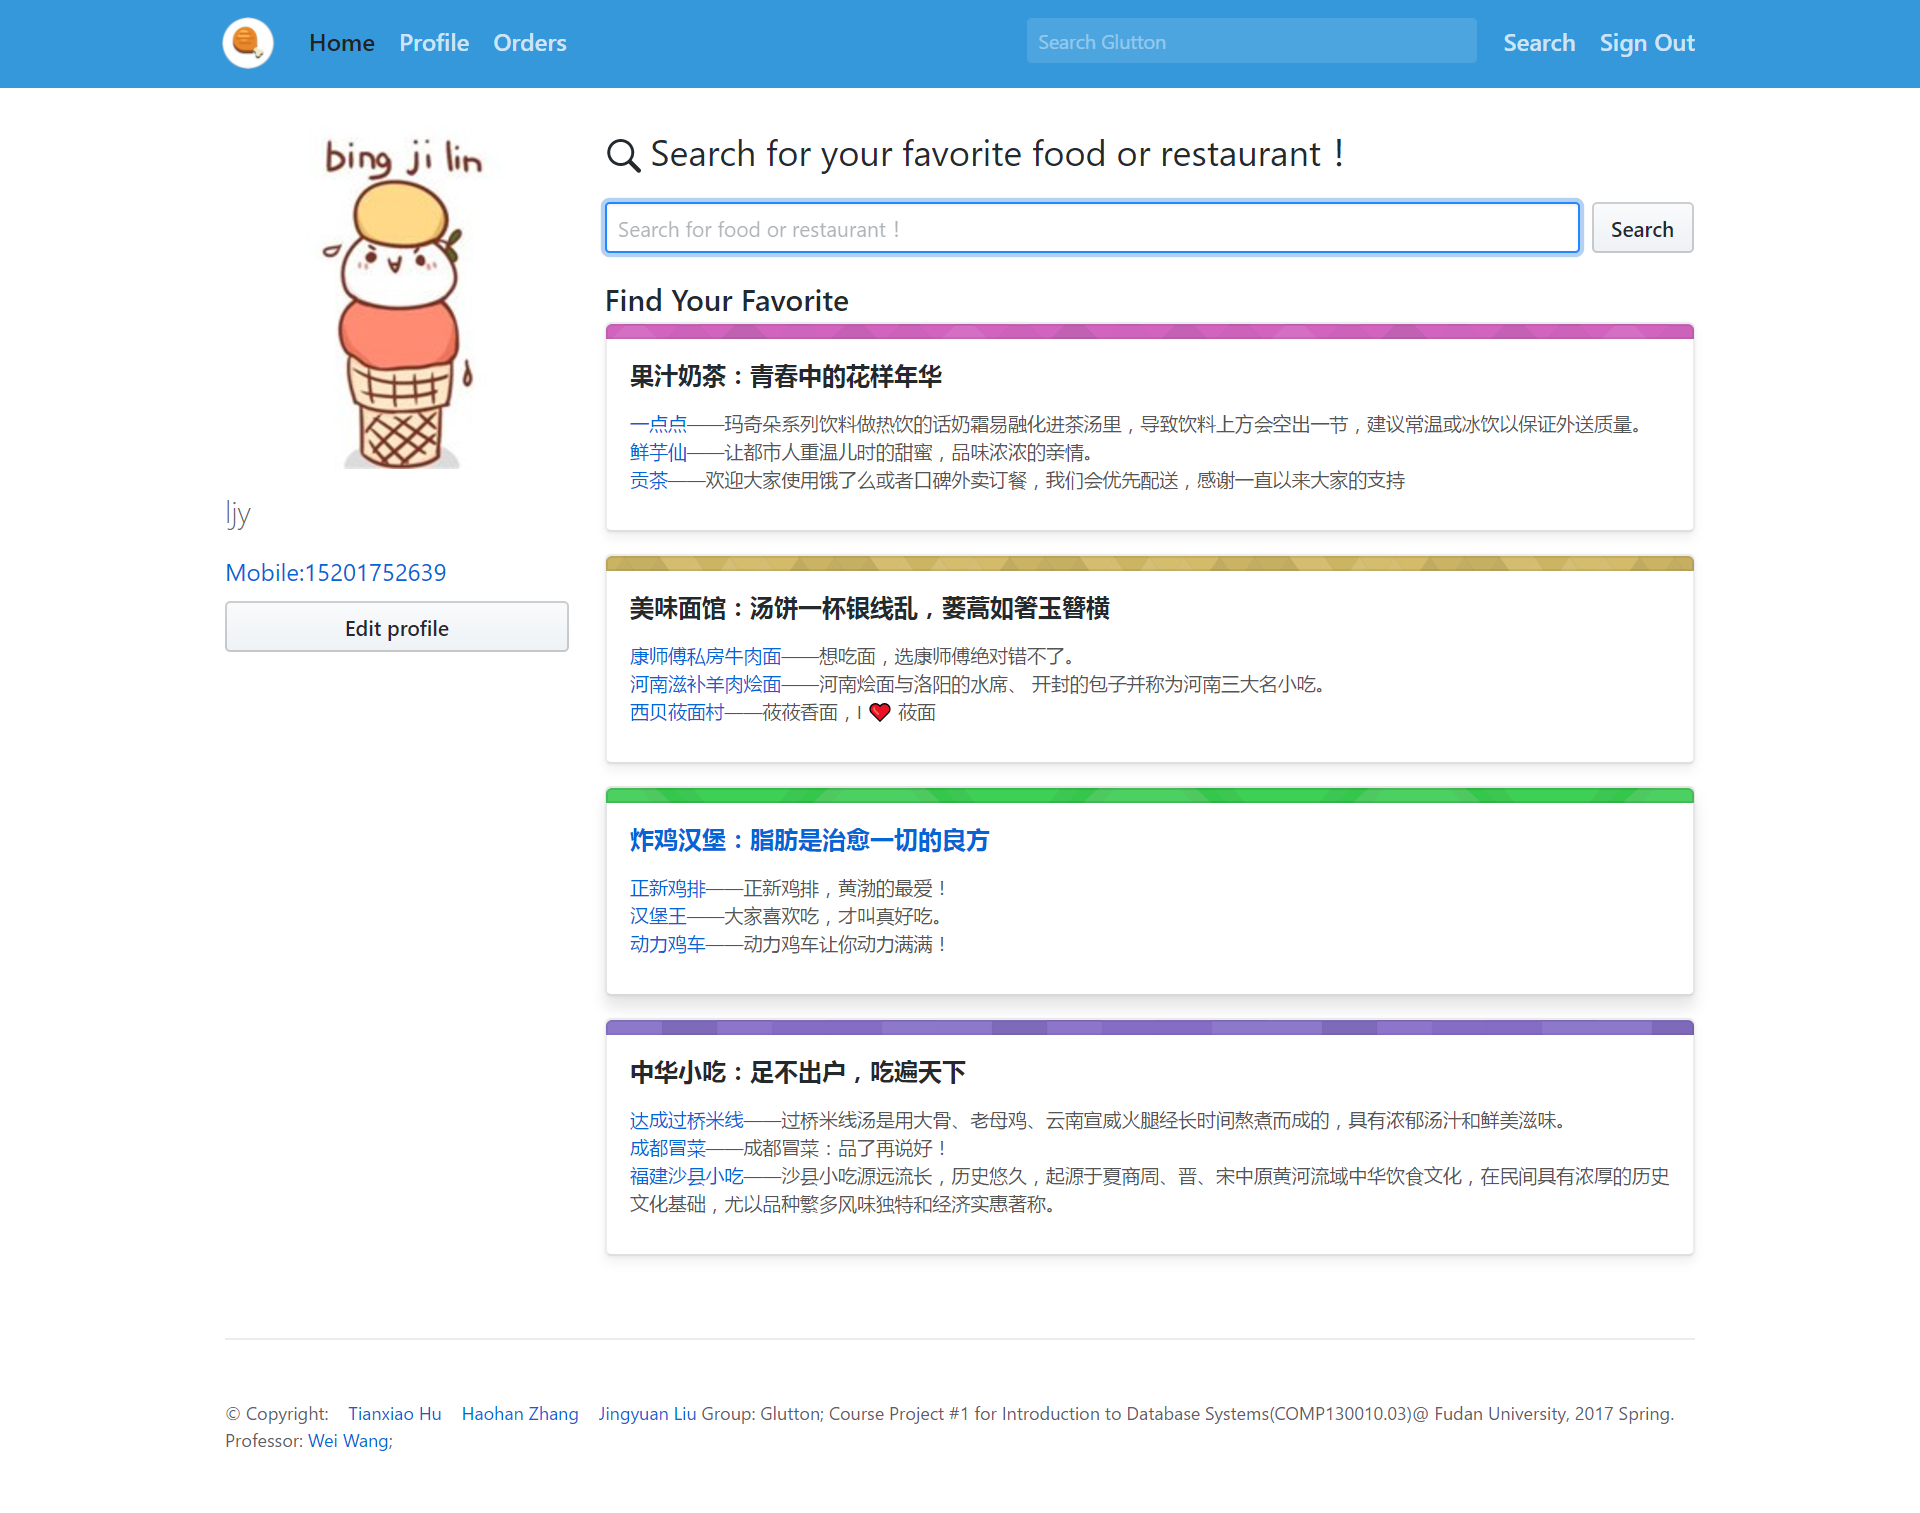
\includegraphics[width=6.00in]{cu-home.png}
     \caption{\small{用户主页}}\label{fig:dummy}
  \end{figure}
  点击Edit profile按钮进入修改个人信息页面,左侧可以选择更改的类型:个人口味偏好,基本信息,更改密码,退出登录。\\
  基本信息可以修改用户名、地址、称呼和个人描述;密码修改,如果修改成功,系统会提示“Succeed”
  \begin{figure}[H]
   \begin{minipage}[t]{0.5\linewidth}
    \centering
     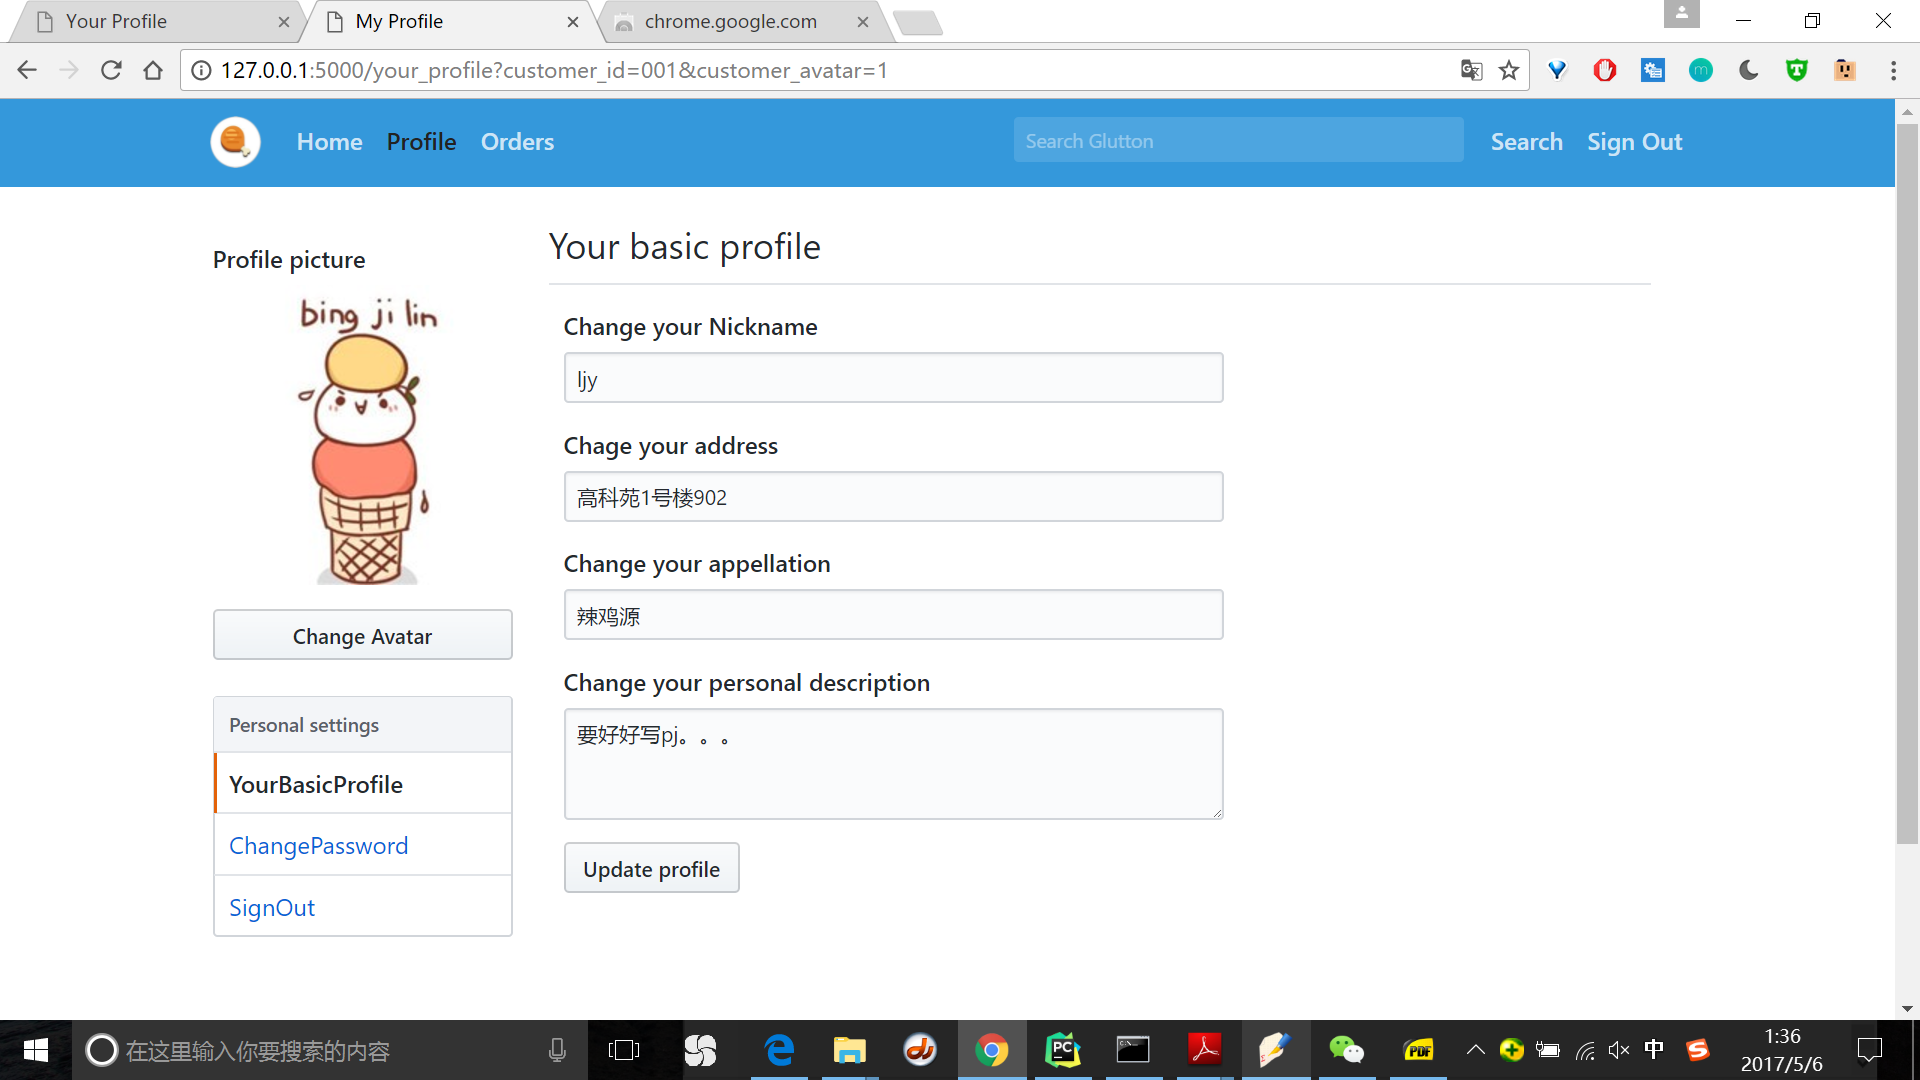
\includegraphics[width=3.2in]{cu-profile.jpg}
     \caption{\small{用户更改信息}}\label{fig:dummy}
   \end{minipage}
   \begin{minipage}[t]{0.5\linewidth}
    \centering
     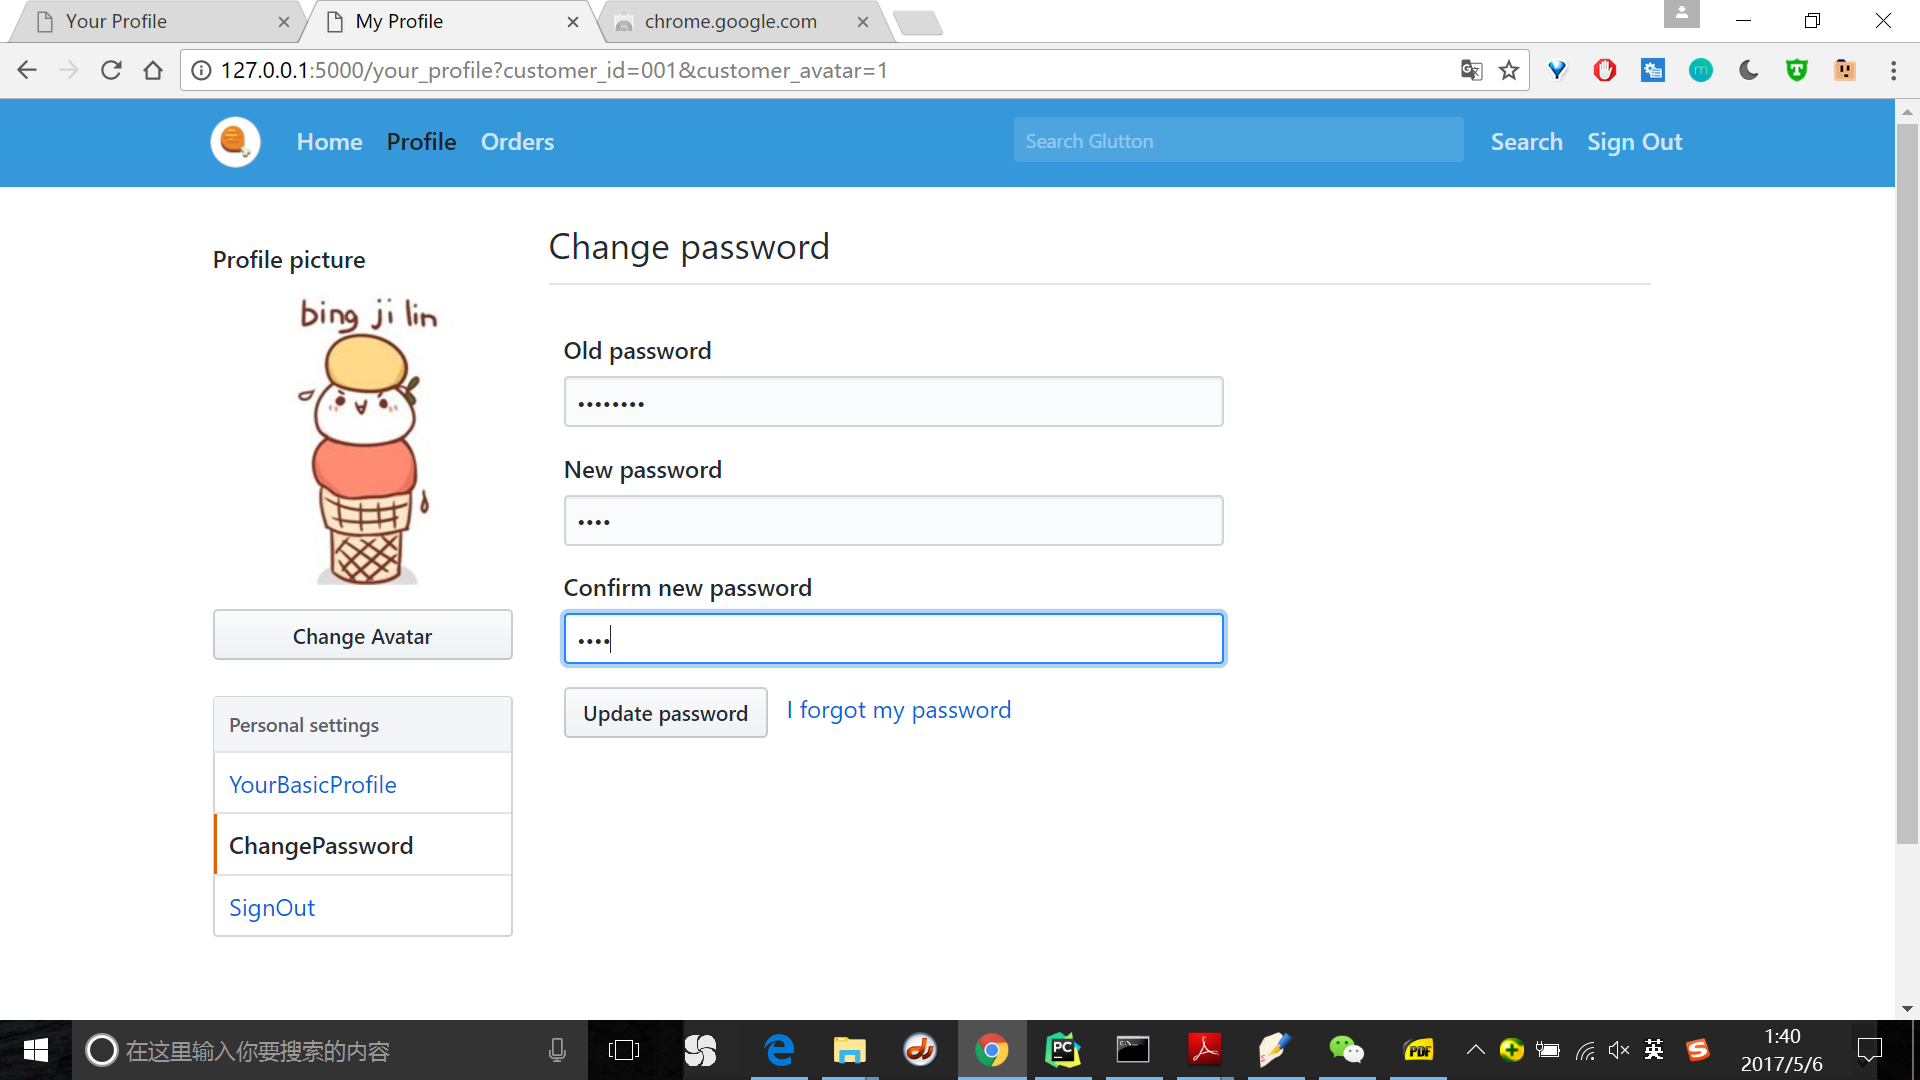
\includegraphics[width=3.2in]{cu-password.jpg}
      \caption{\small{用户更改密码}}\label{fig:dummy}
   \end{minipage}
   \end{figure}
   用户可以点击图片,修改个人口味偏好。共有9中偏好类型供选择,任意点击一个,系统会提示转换成功,页面跳转至个人主页,可以看到口味头像已有变化。
   \begin{figure}[H]
   \centering
     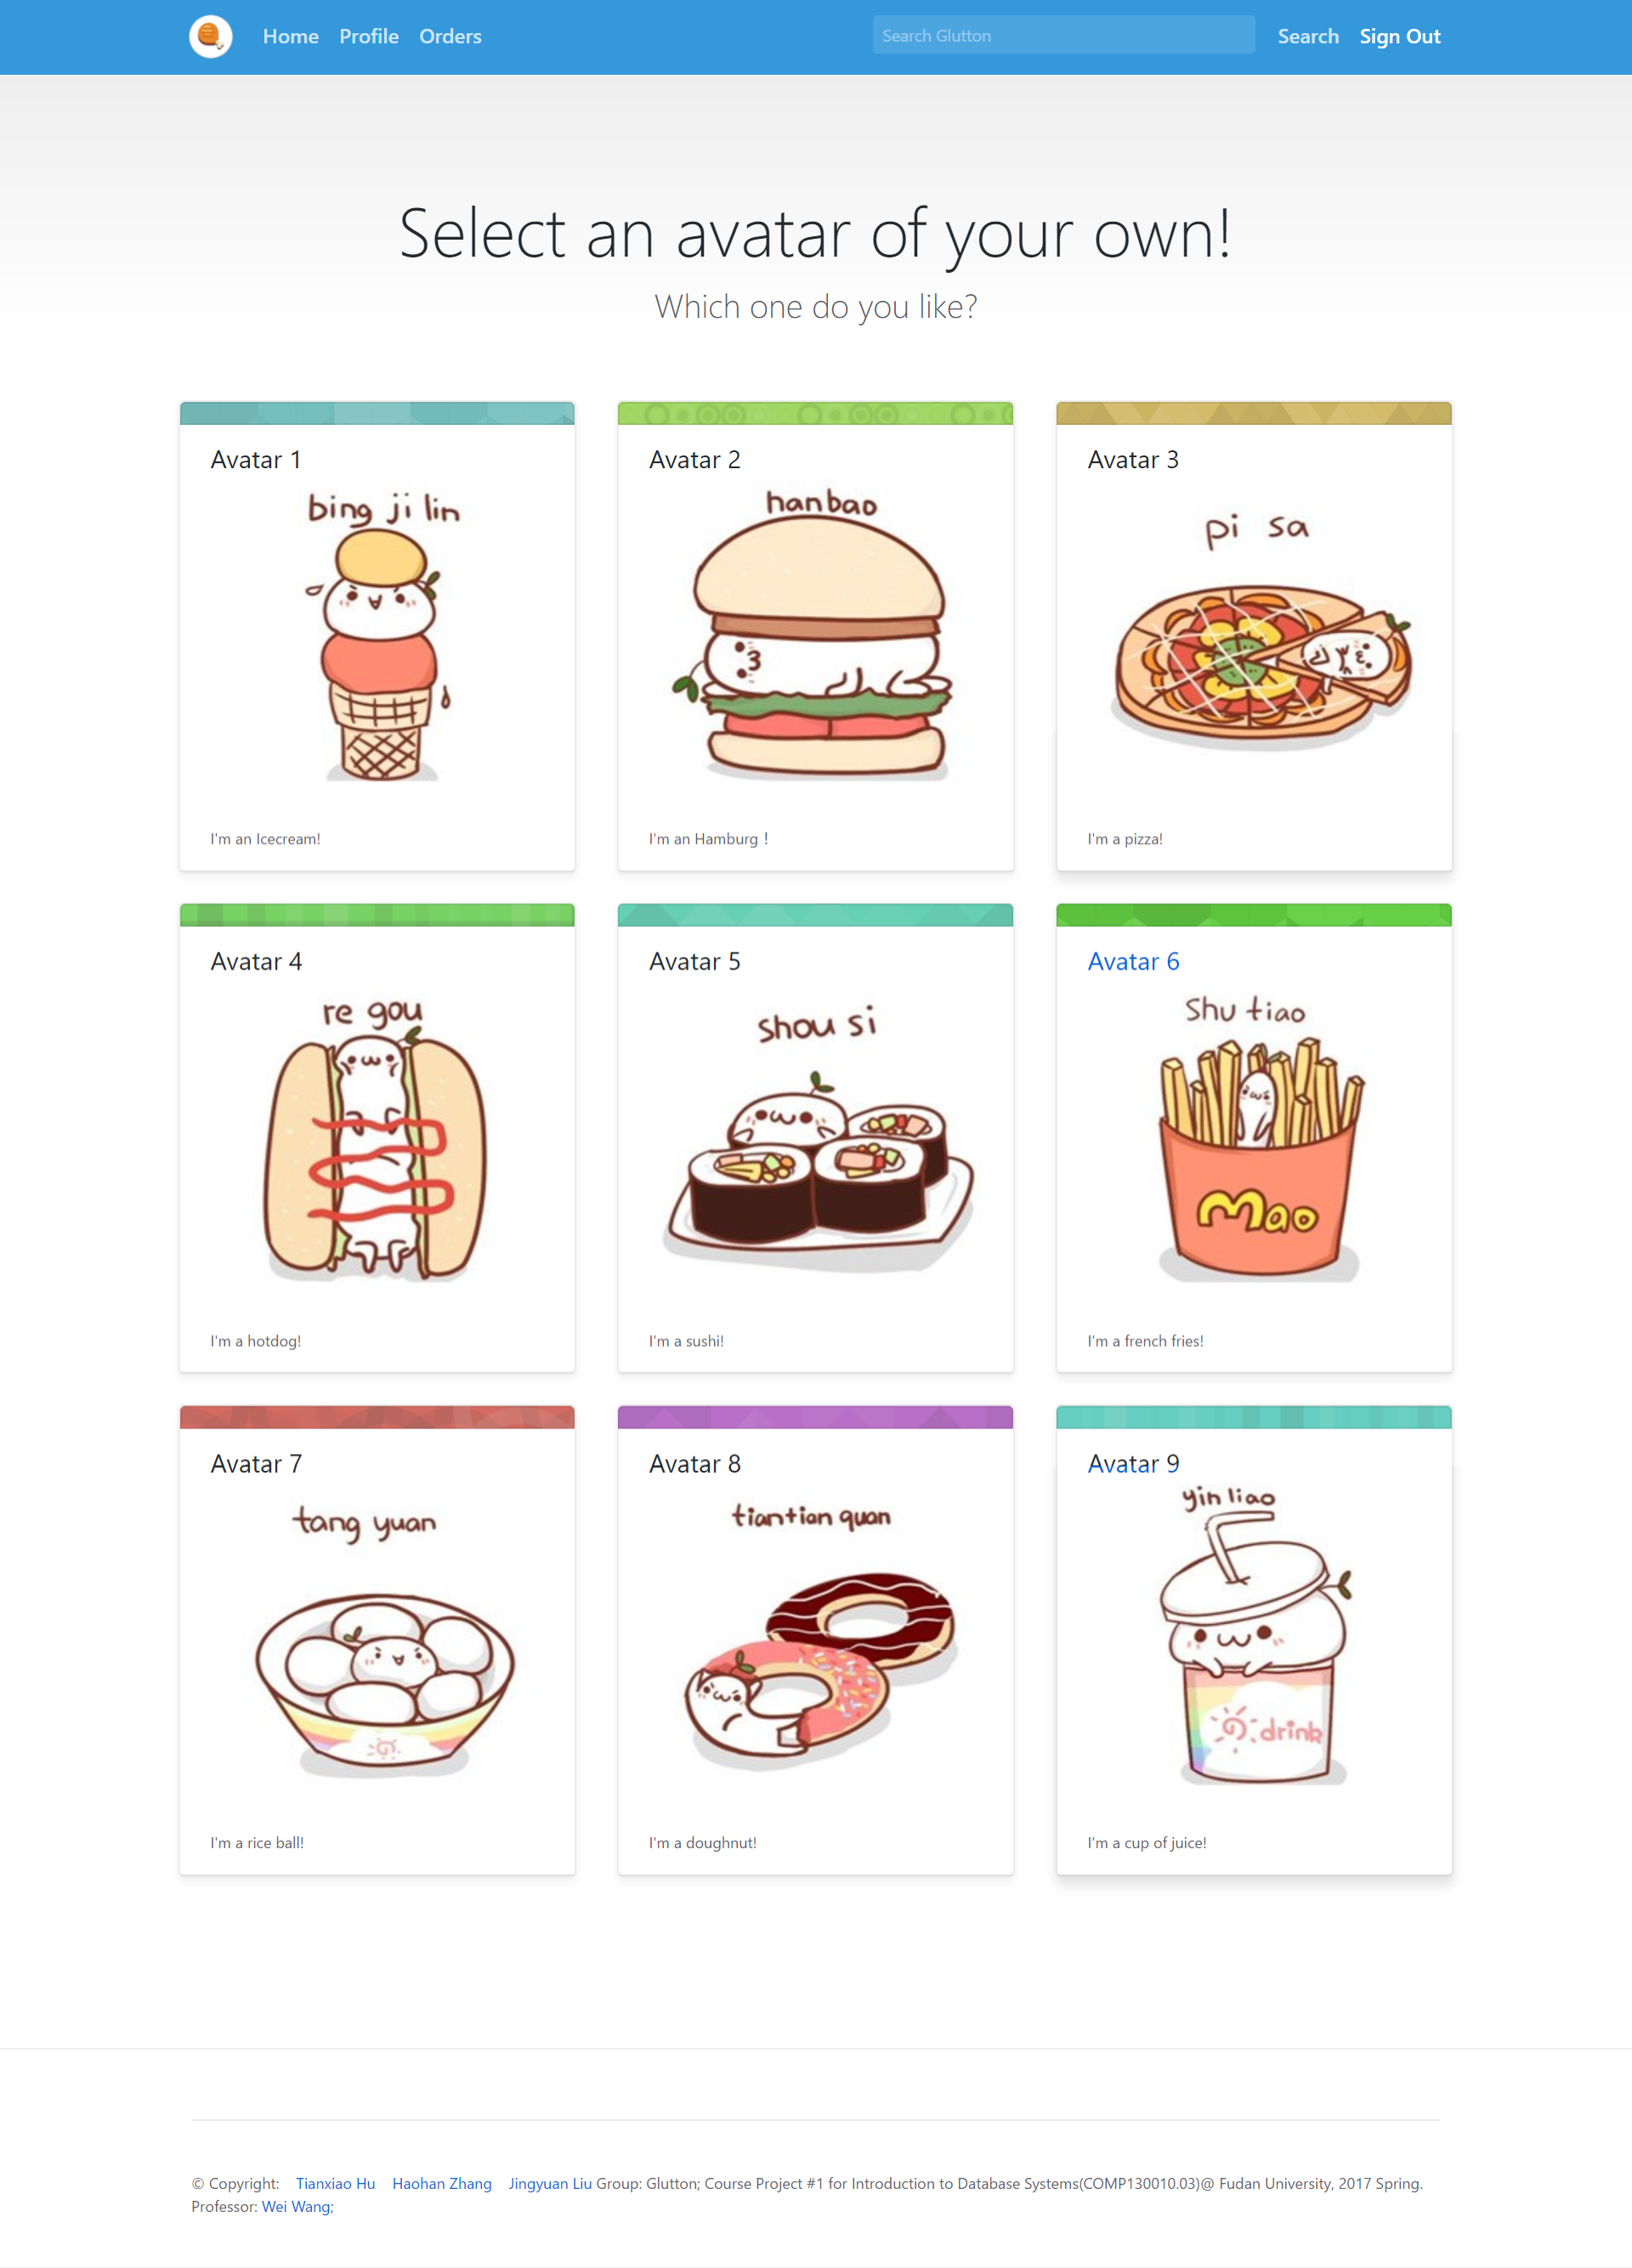
\includegraphics[width=6.00in]{avatar.png}
     \caption{\small{用户口味选择}}\label{fig:dummy}
  \end{figure}
  \item 查找商家\\
  在搜索框中输入商家的名称,例如“一点点”,可以查询到对应商家信息。点击可以进入商家。\\
  还可以按照随机、月销量、起送费顺序查看商家列表,右侧有查询历史记录。\\
  同样在商家内,可以按照随机、月销量、商品价格顺序查看菜品列表。
  \begin{figure}[H]
   \centering
     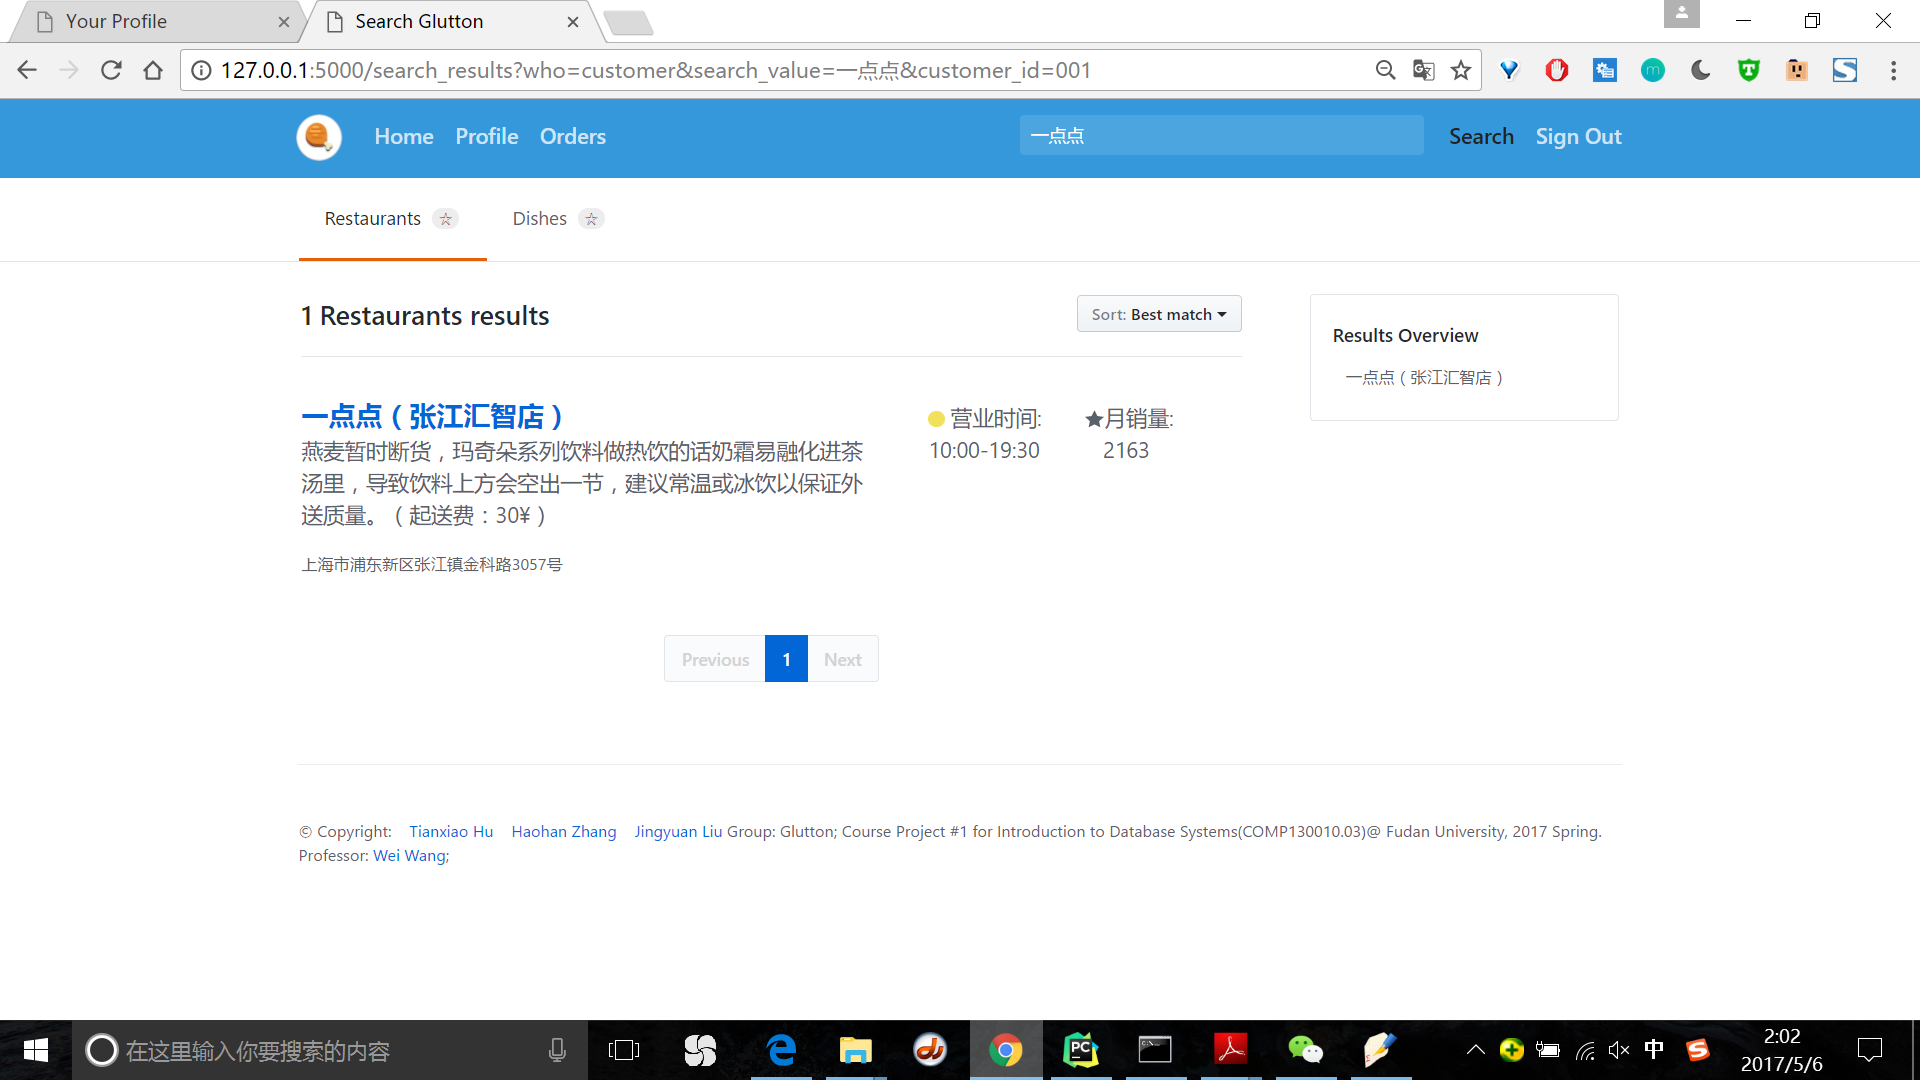
\includegraphics[width=6.00in]{cu-se-re.jpg}
     \caption{\small{用户查找特定商家}}\label{fig:dummy}
  \end{figure}
  \begin{figure}[H]
   \centering
     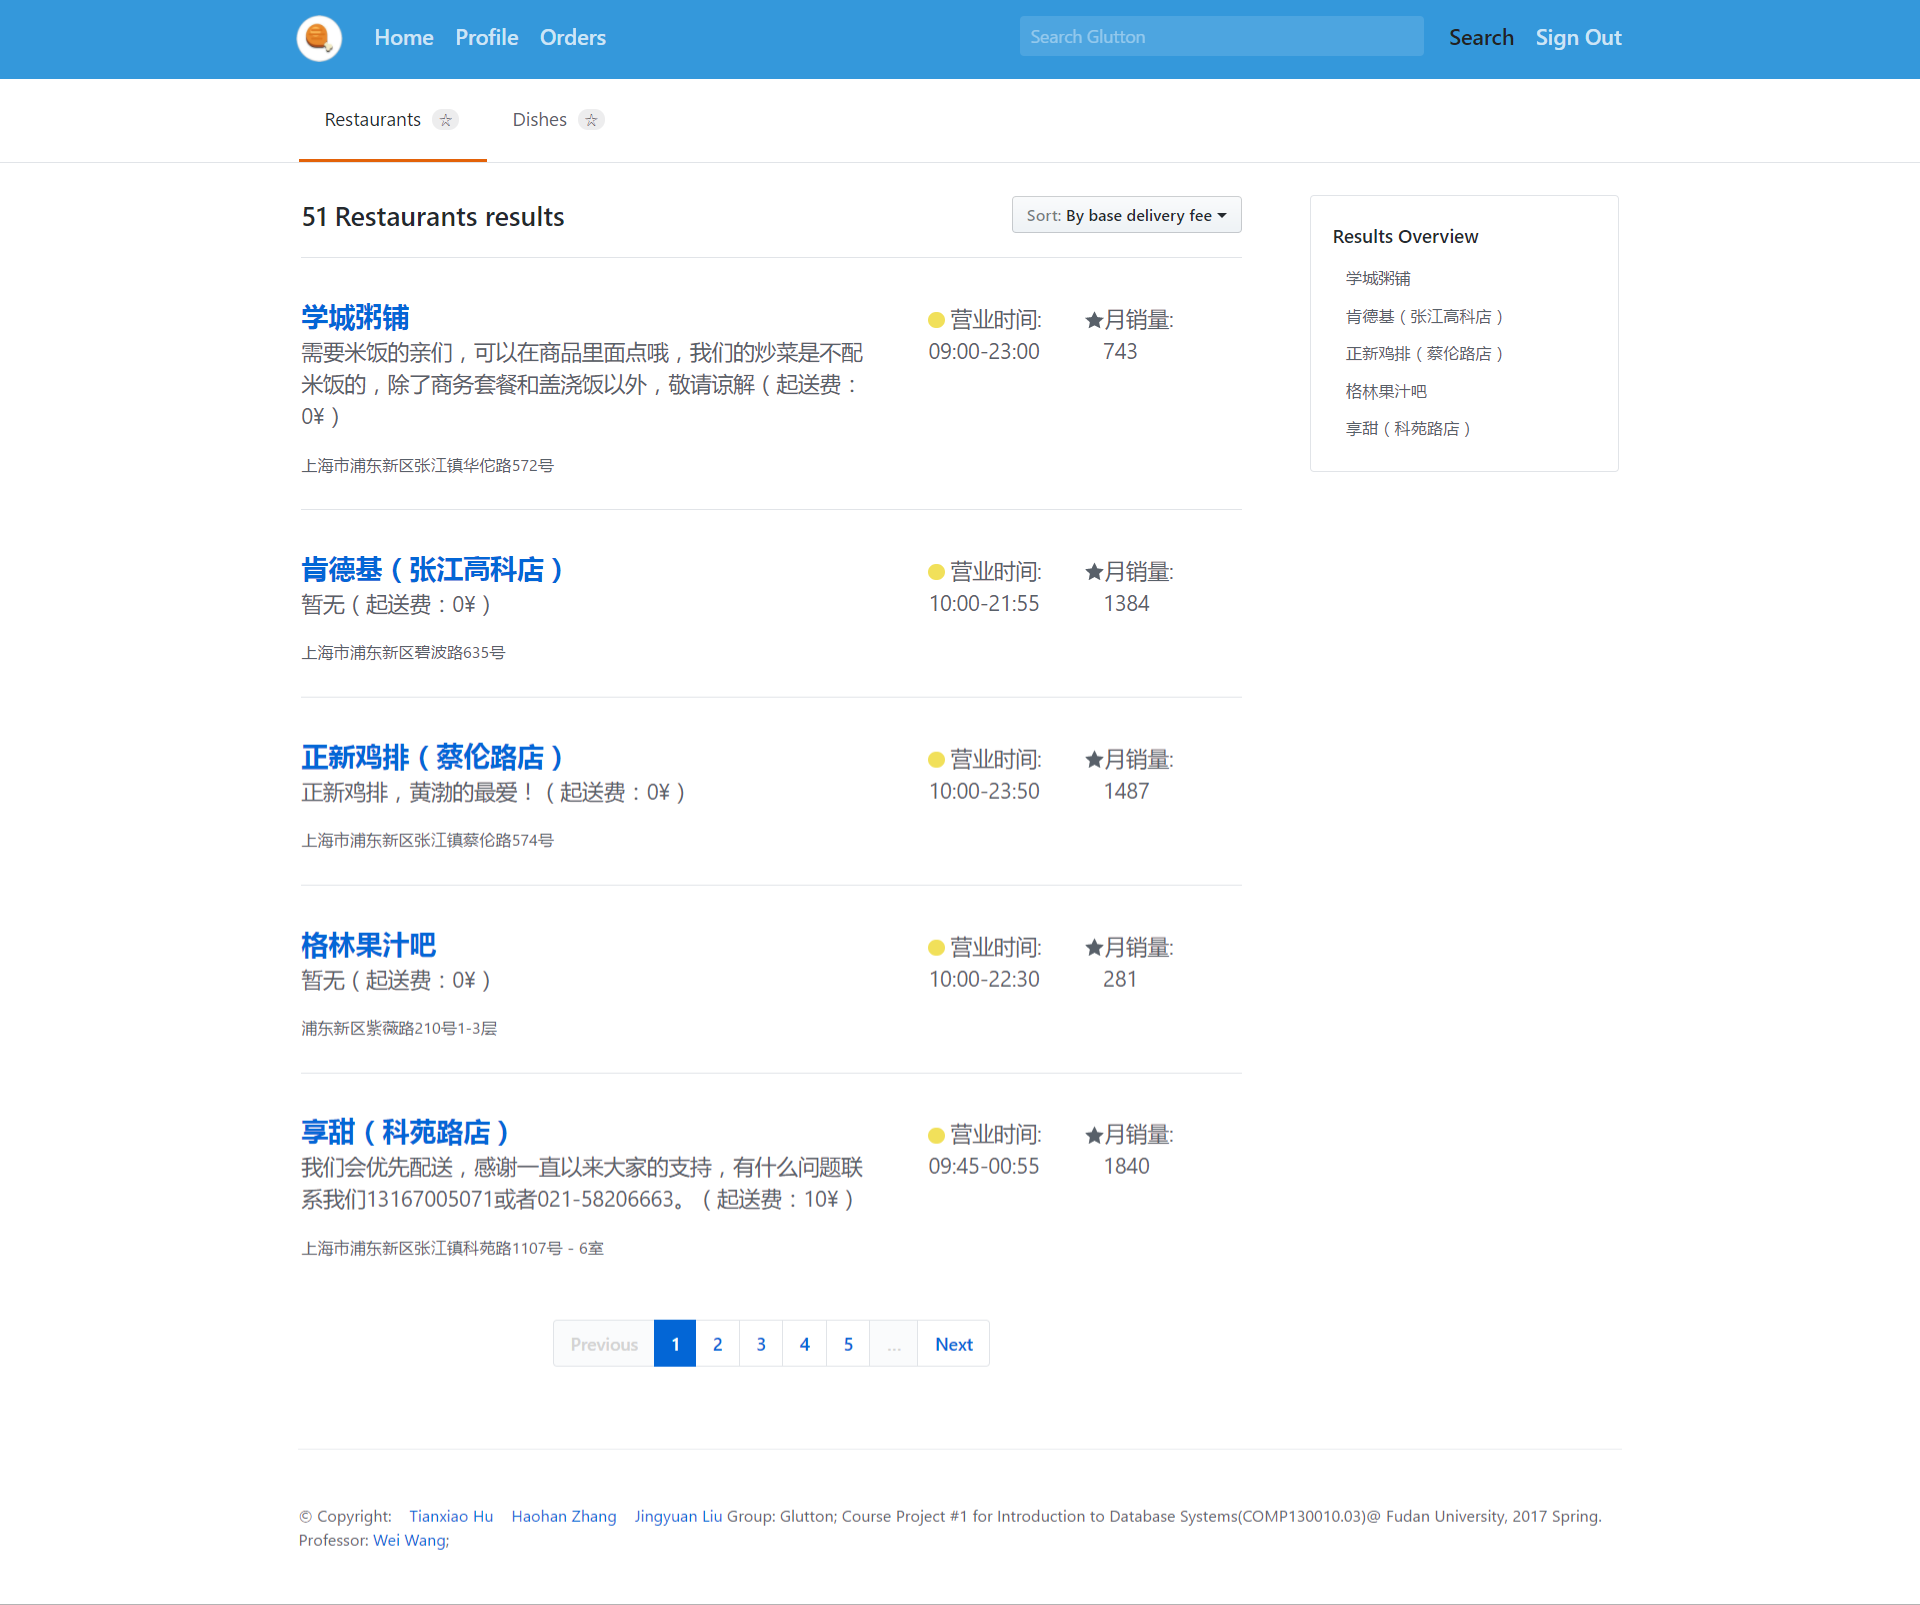
\includegraphics[width=6.00in]{cu-re.png}
     \caption{\small{用户查看商家列表}}\label{fig:dummy}
  \end{figure}
  \item 下单\\
  跳转到商家页面,显示所有菜品,对每个菜品可以选择添加或删除,最后点击Submit Order提交订单。系统提示订单提交成功。
  \begin{figure}[H]
   \centering
     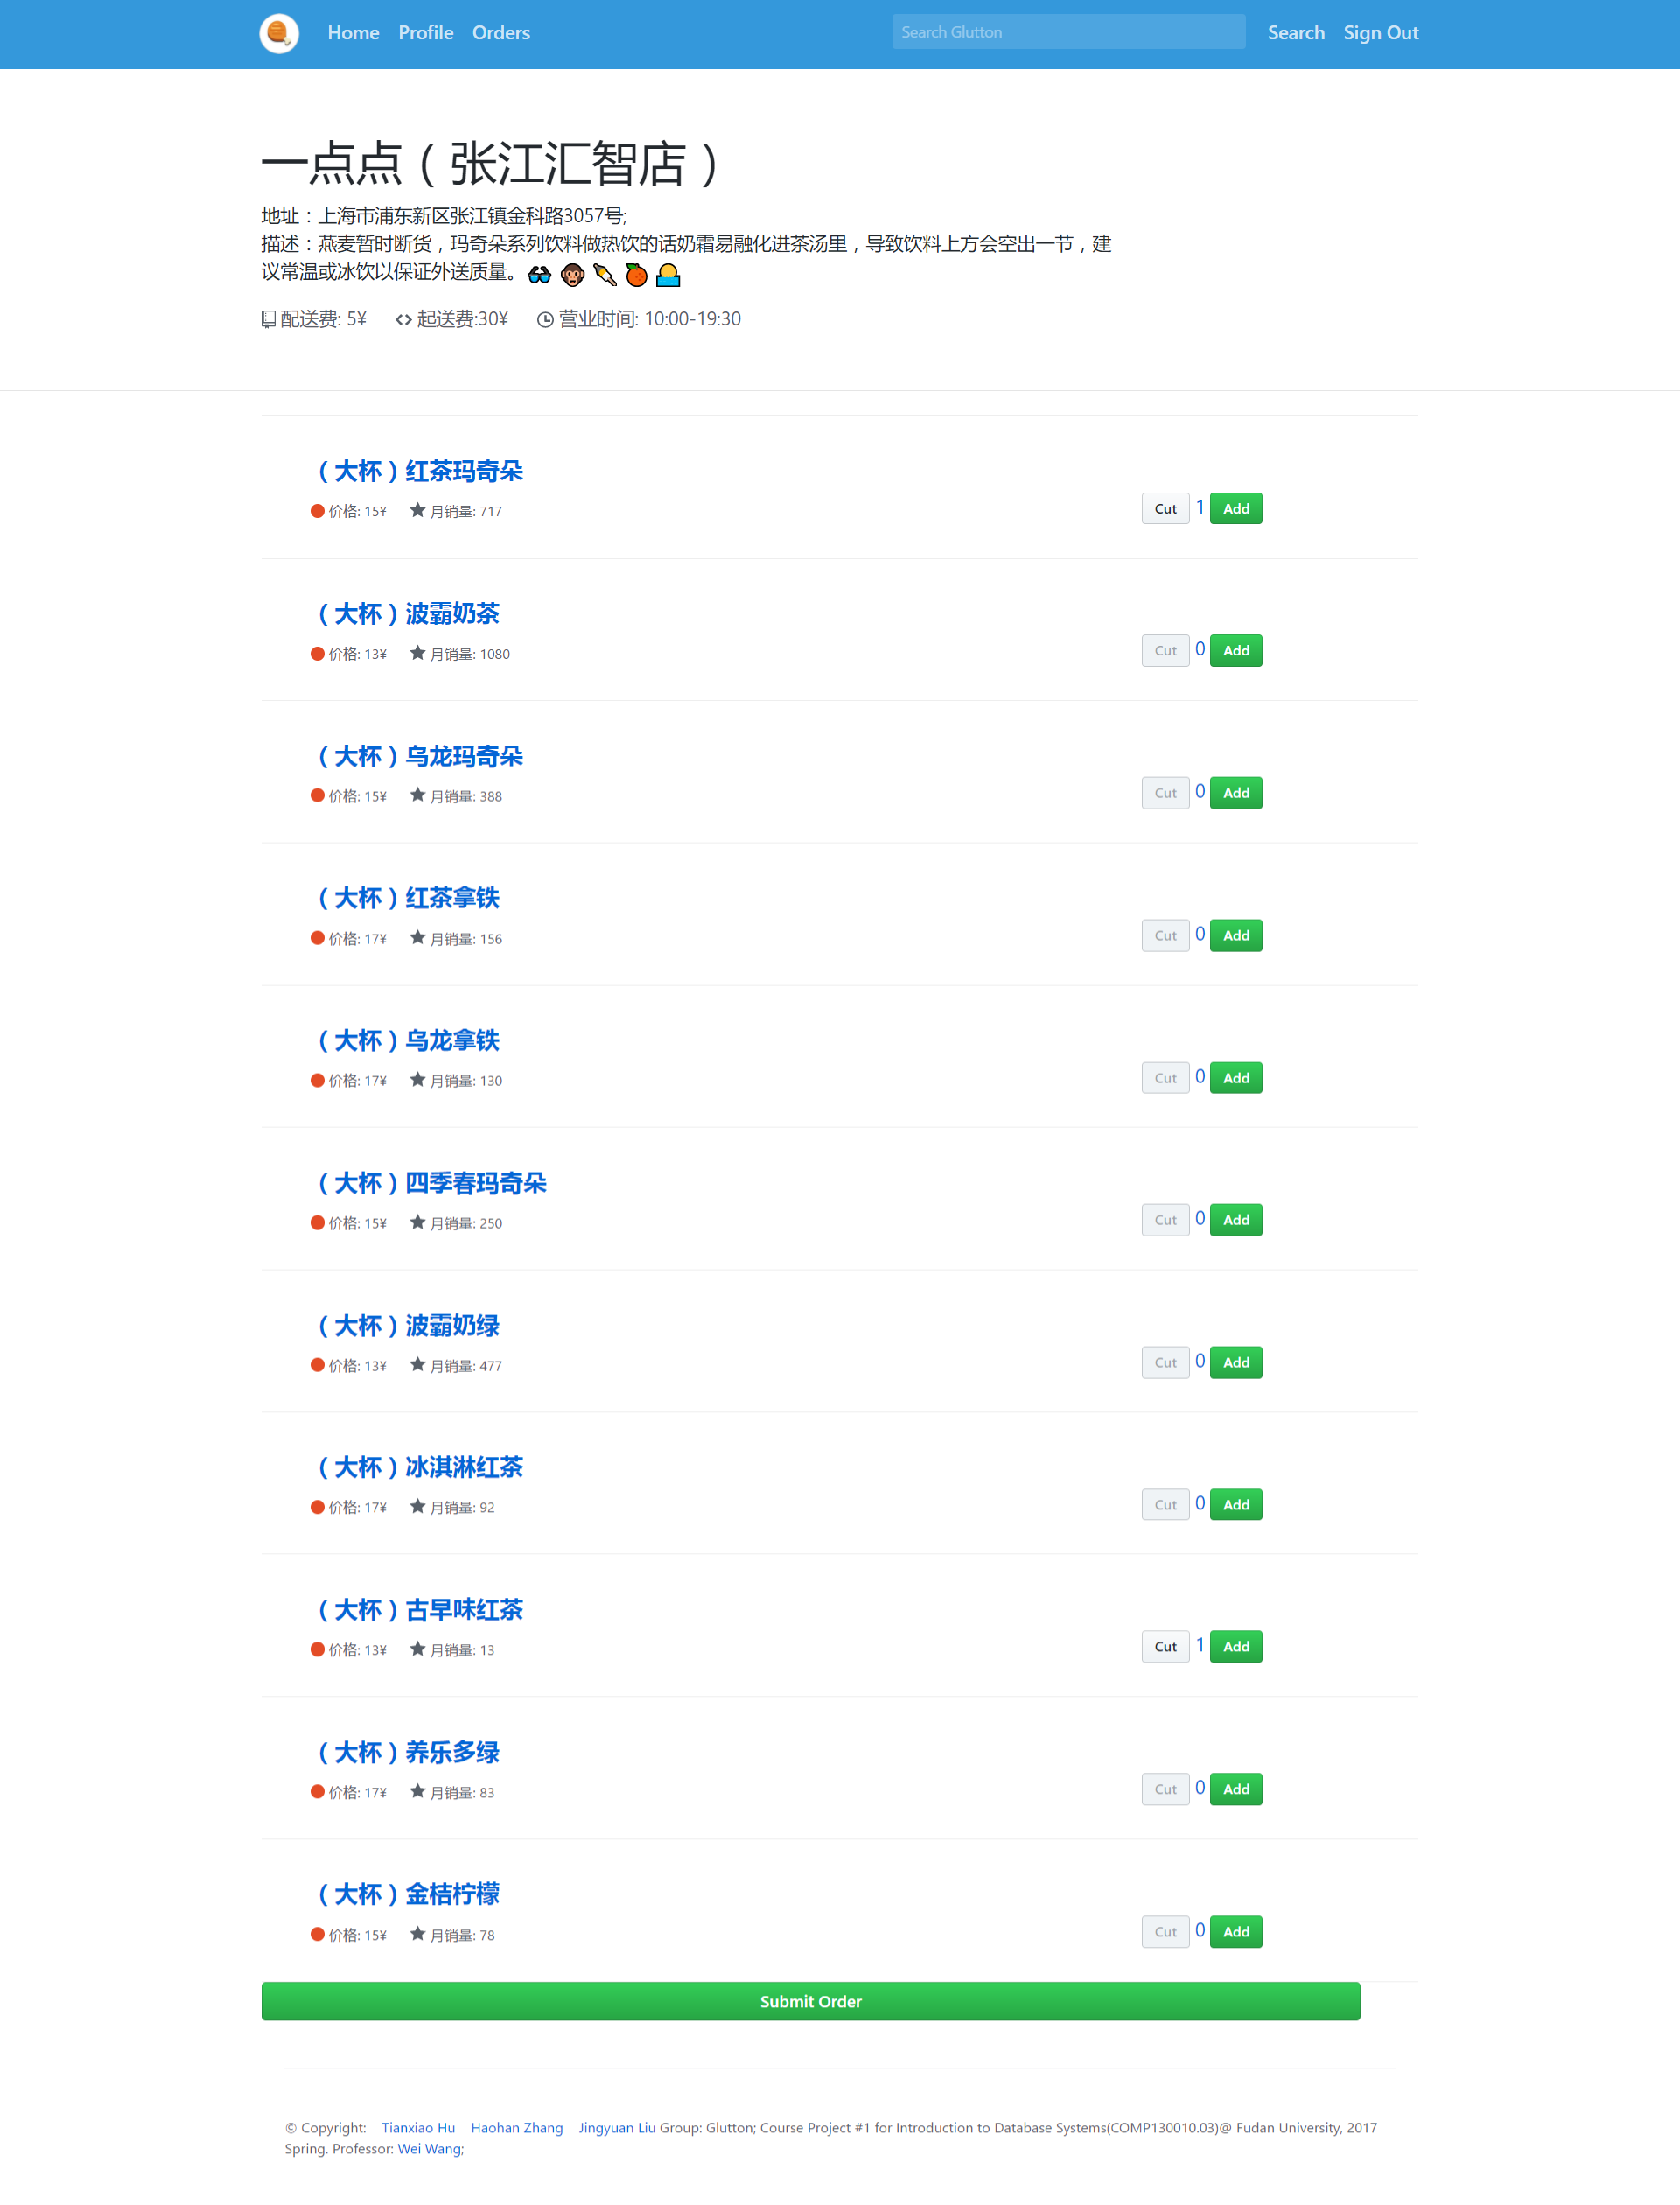
\includegraphics[width=6.00in]{cu-dish.png}
     \caption{\small{用户下单}}\label{fig:dummy}
  \end{figure}
  \item 收货\\
  点击order按钮,跳转到订单页面,可以查看所有订单信息。点击Received the Dishes确认收货。
  \begin{figure}[H]
   \centering
     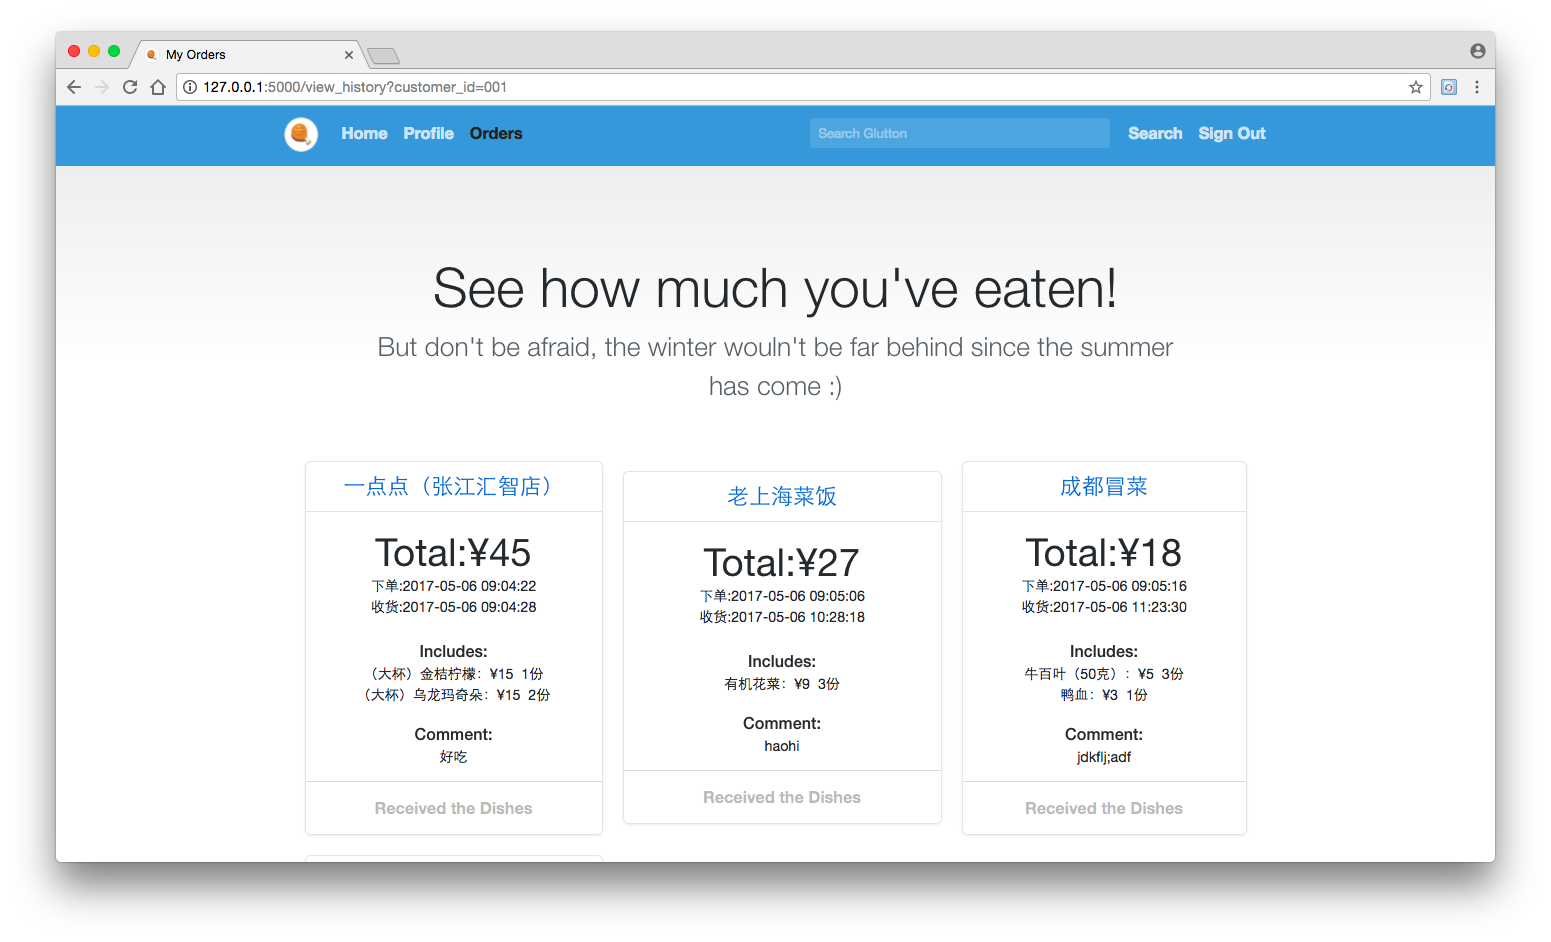
\includegraphics[width=6.00in]{cu-order.jpg}
     \caption{\small{用户查看订单确认收货}}\label{fig:dummy}
  \end{figure}
  \item 评论\\
  点击确认收货按钮后,会弹出评价窗口,用户可以写评价,系统提示提交评价成功,跳转到订单界面。
  \begin{figure}[H]
   \centering
     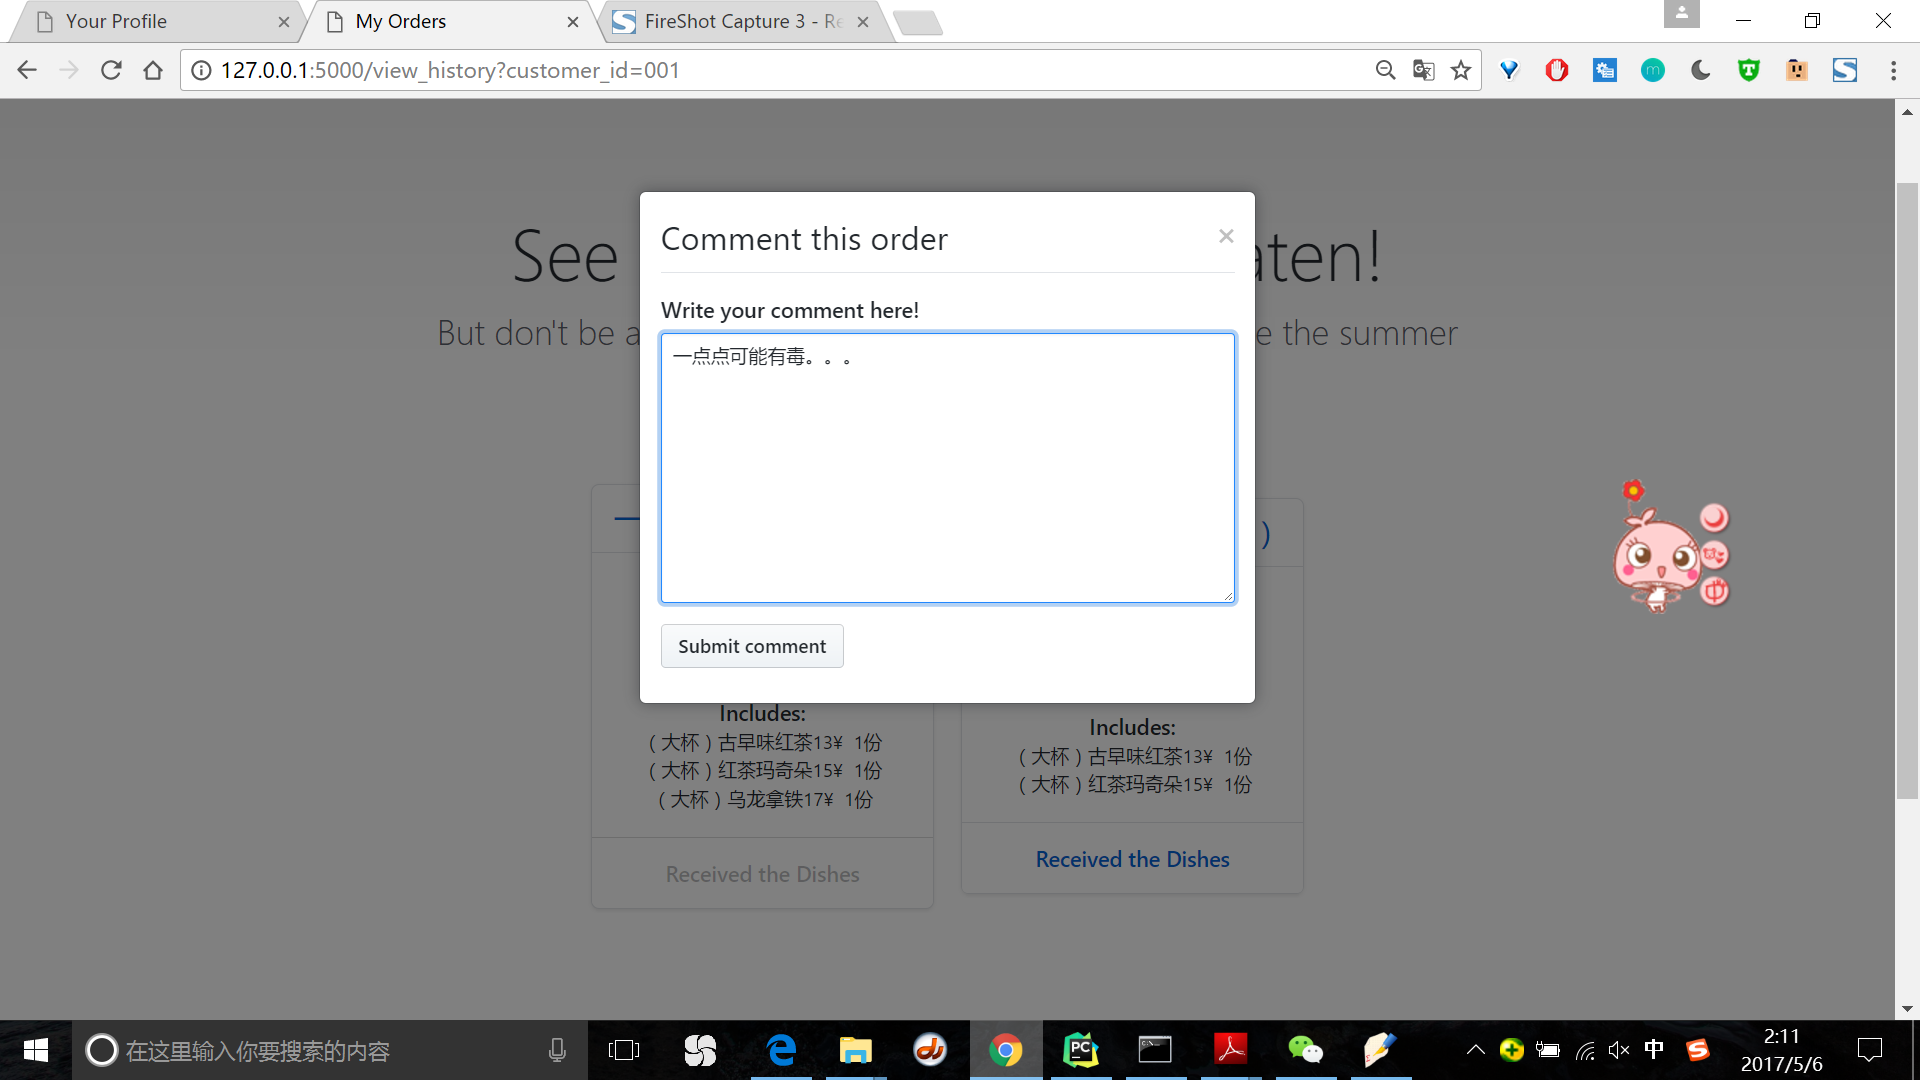
\includegraphics[width=6.00in]{cu-comment.jpg}
     \caption{\small{用户填写评价}}\label{fig:dummy}
  \end{figure}
  \end{itemize}
  
 \subsection{针对商家的功能}
 商家主界面与用户类似,右侧和中部为登录商家和注册商家按钮。
 \begin{figure}[H]
   \centering
     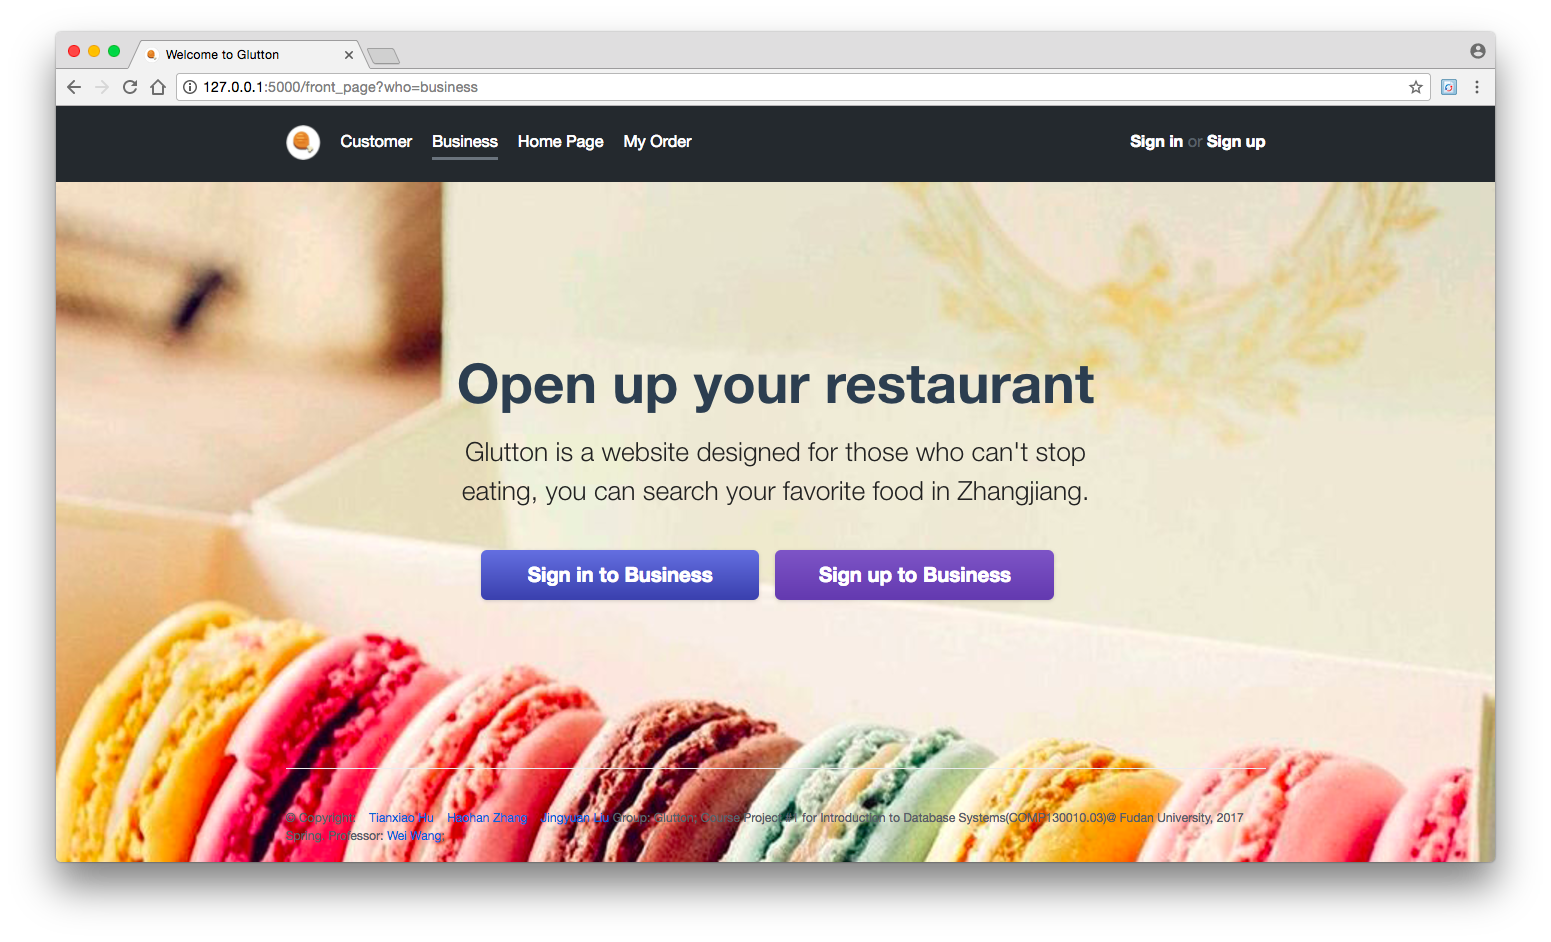
\includegraphics[width=6.00in]{re-front.png}
     \caption{\small{主页面}}\label{fig:dummy}
  \end{figure}
  \begin{itemize}
  \item 注册/登录\\
  点击sign up to business按钮我们进入商家注册页面,输入用户名,店铺名,密码来注册。\\
  点击sign in to business按钮我们进入商家登录页面,用用户名和密码登录。如果密码输入错误,系统会提示密码或用户名错误。
  \begin{figure}[H]
   \begin{minipage}[t]{0.5\linewidth}
    \centering
     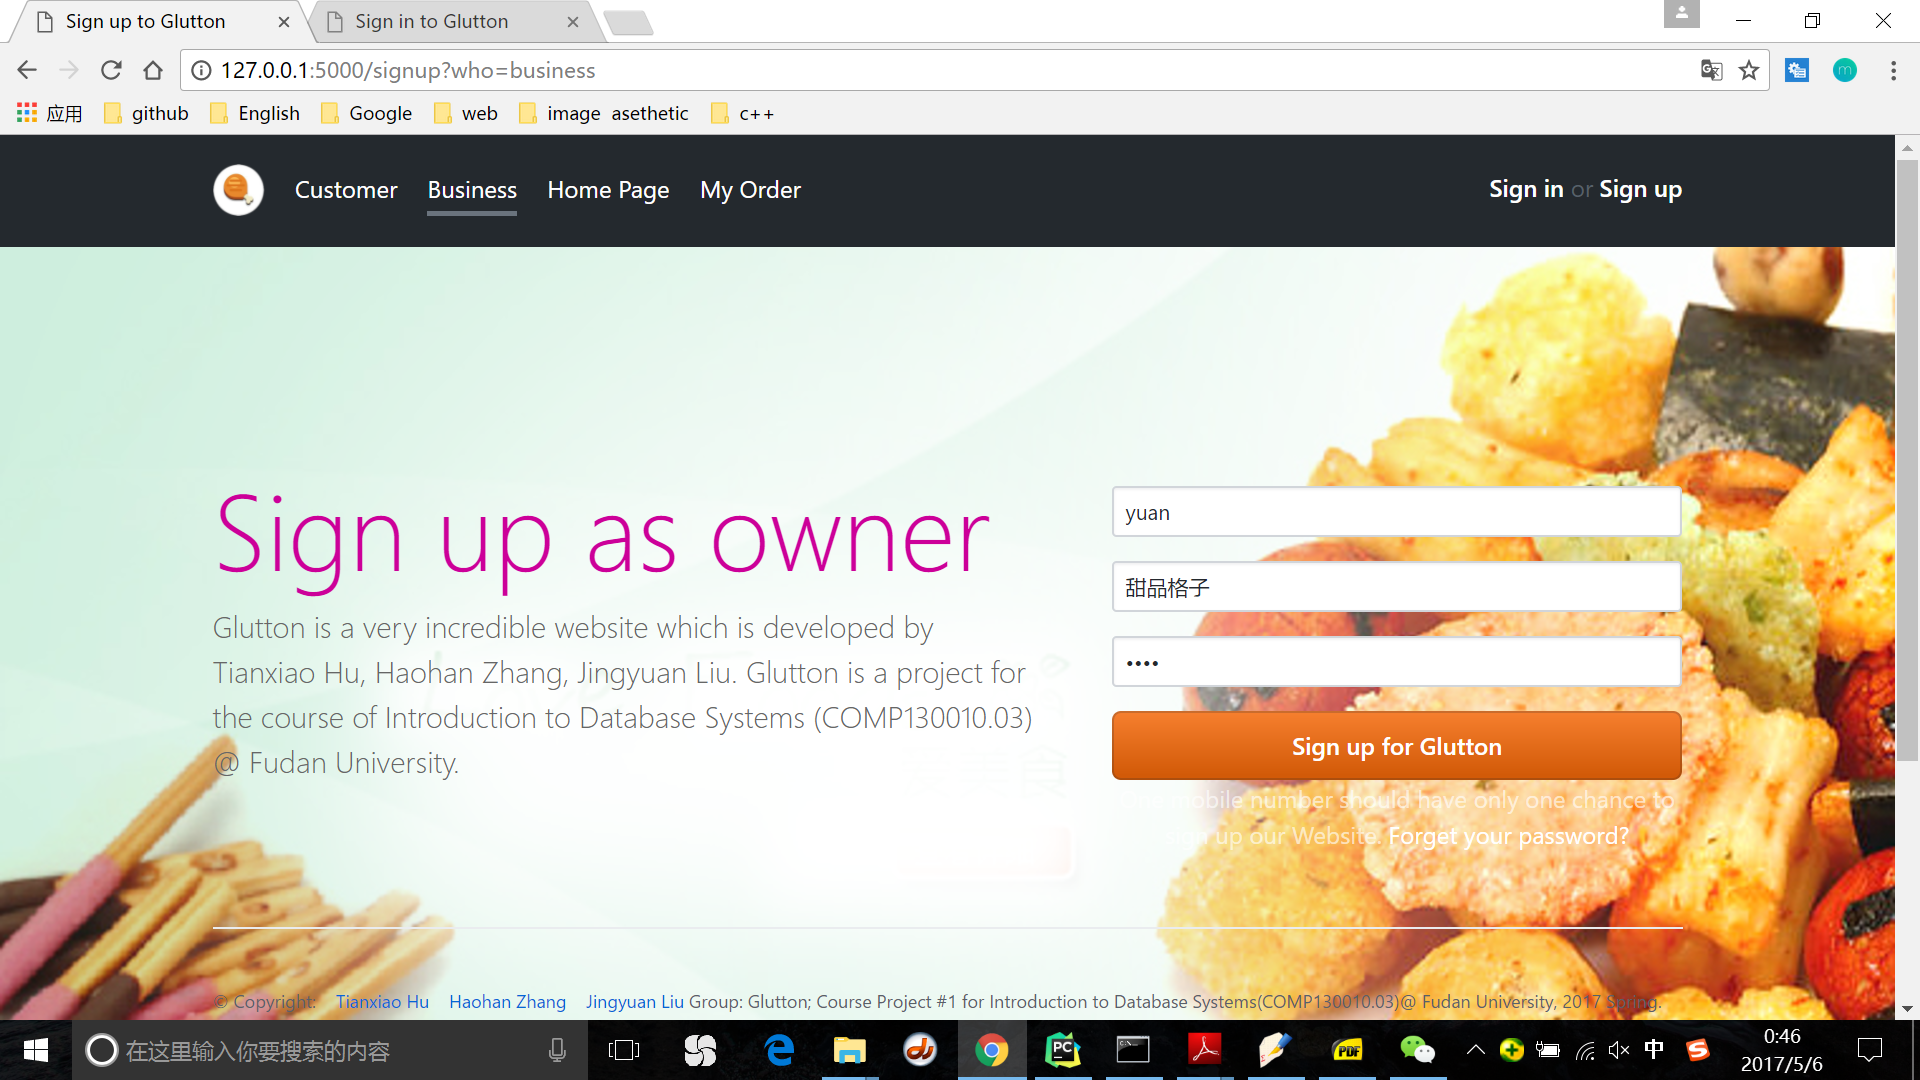
\includegraphics[width=3.2in]{re-signup.jpg}
     \caption{\small{商家注册}}\label{fig:dummy}
   \end{minipage}
   \begin{minipage}[t]{0.5\linewidth}
    \centering
     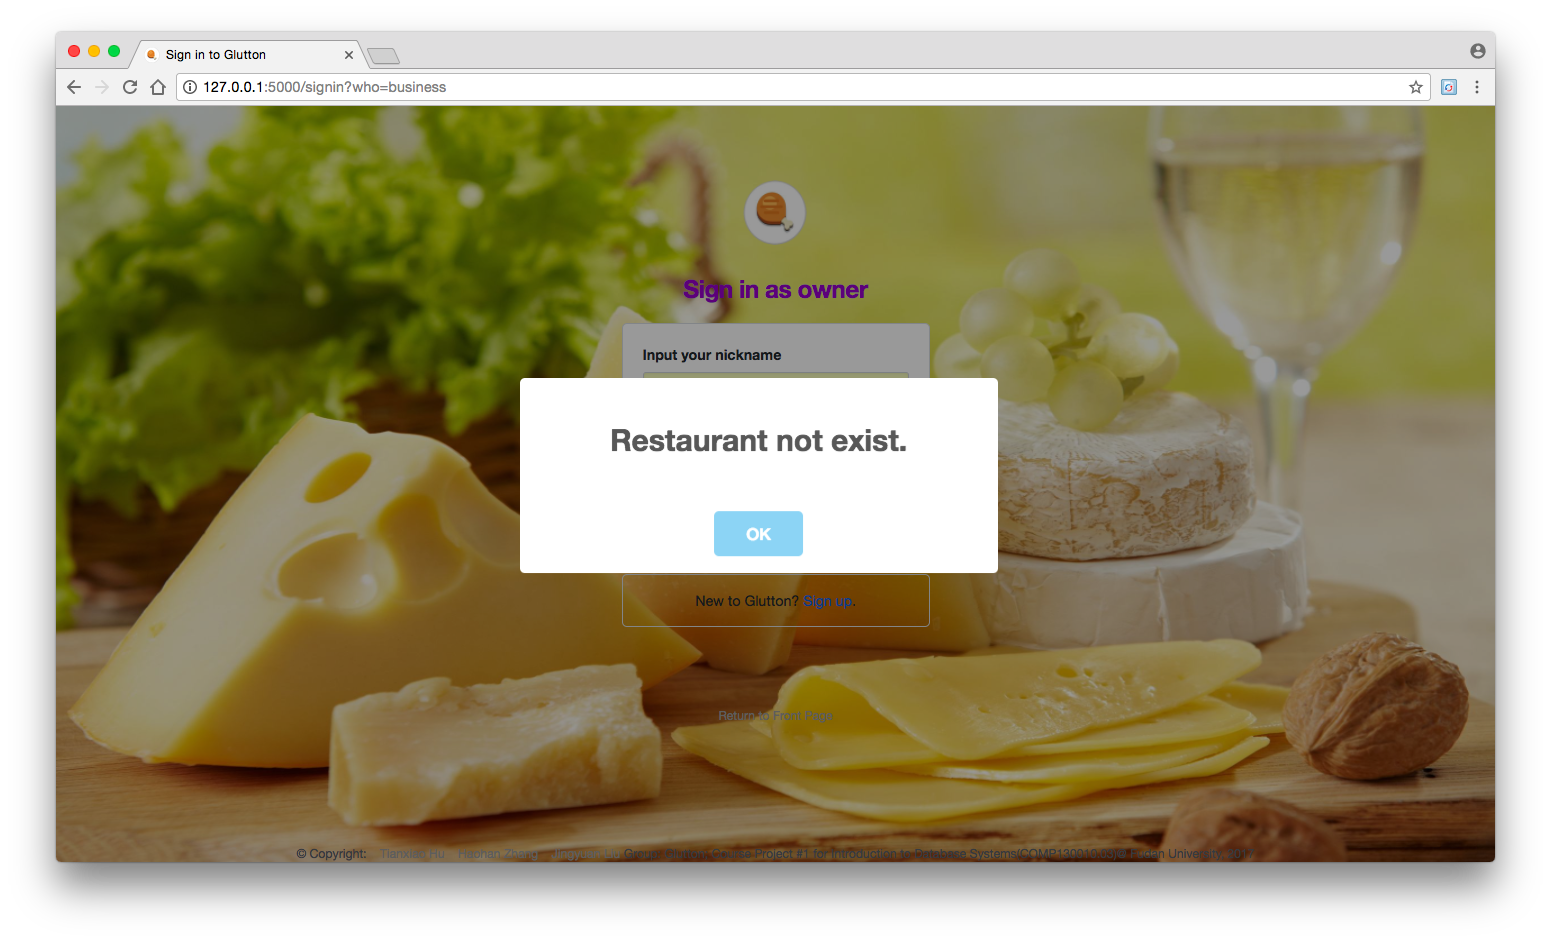
\includegraphics[width=3.2in]{re-signin.jpg}
      \caption{\small{商家登录}}\label{fig:dummy}
   \end{minipage}
   \end{figure}
  \item 更改信息\\
  登录成功后,我们进入到商家的主页。主页的最上方是导航栏,左侧四个按钮可以选择主页,商家信息,菜品,订单。右侧有搜索栏和退出登录按钮。\\
  左侧显示用户名和商家号,及修改商家信息按钮。
  \begin{figure}[H]
   \centering
     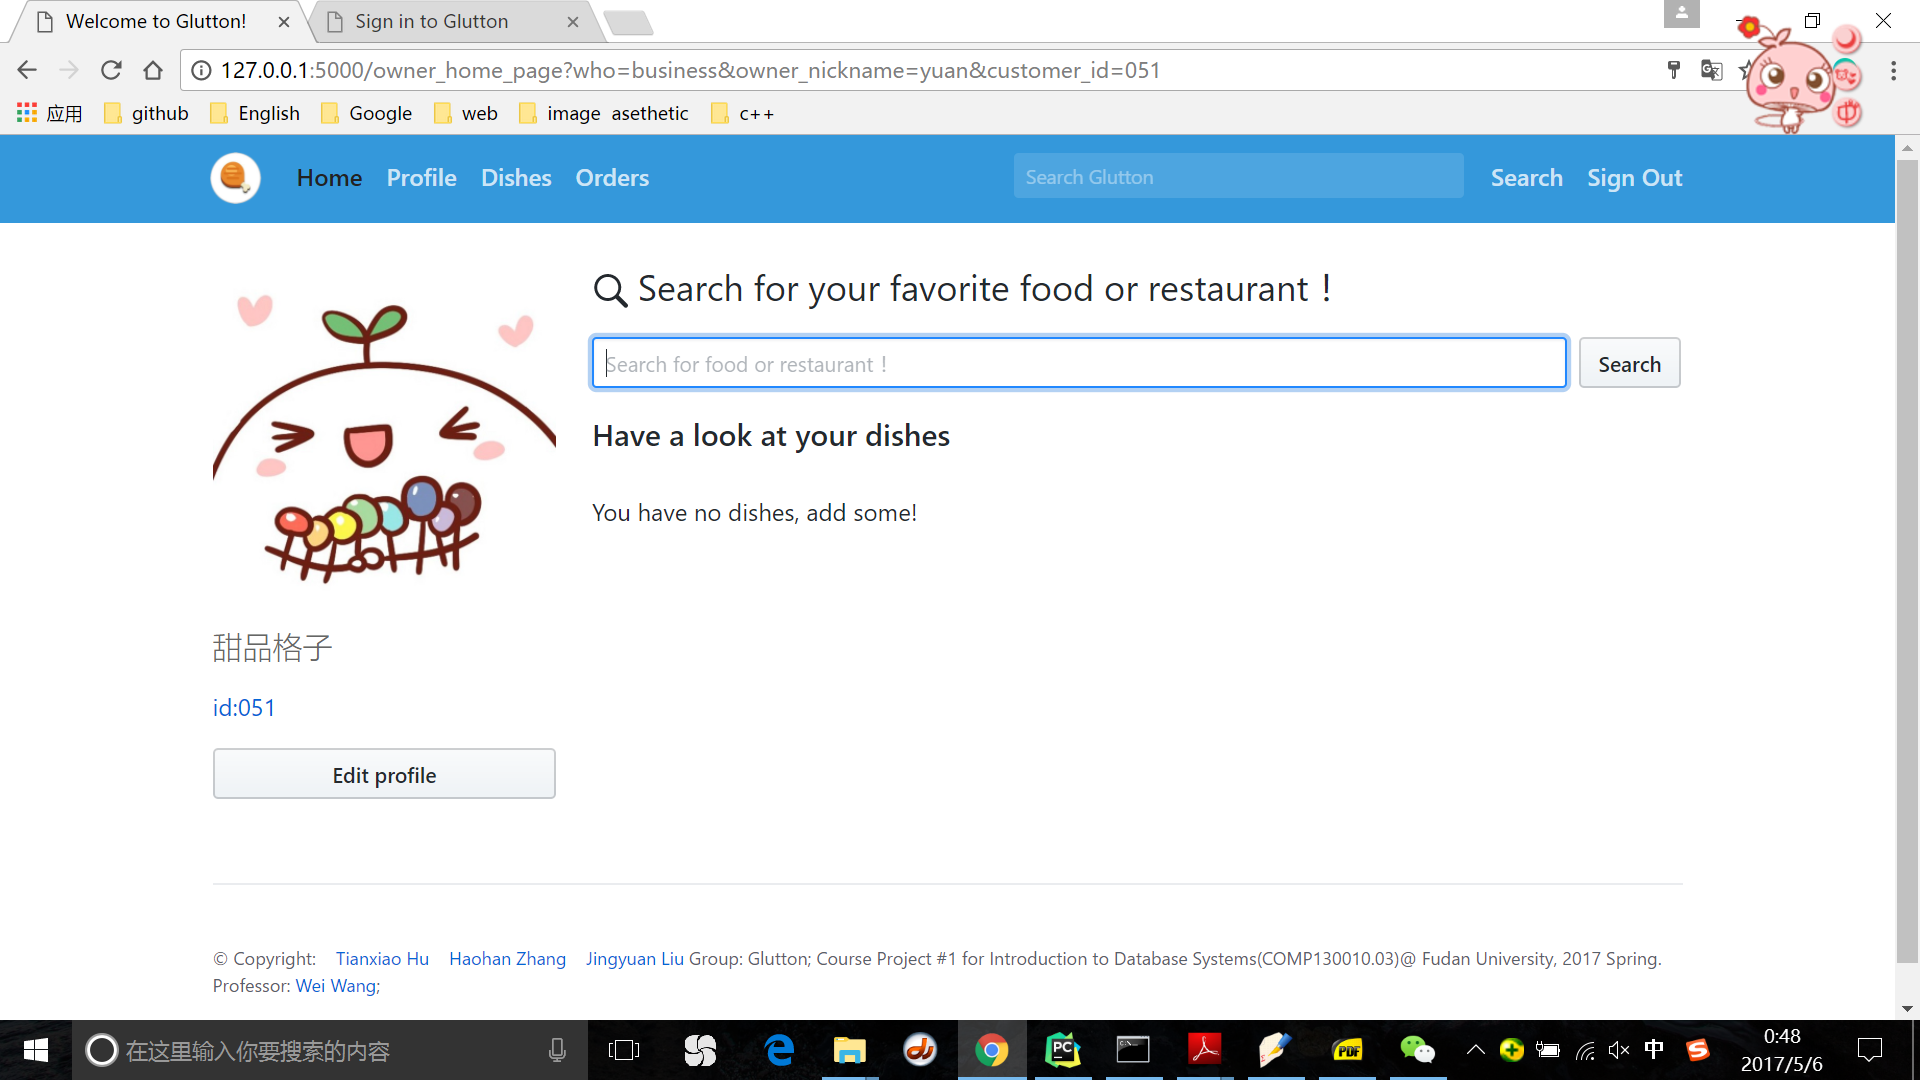
\includegraphics[width=6.00in]{re-home.jpg}
     \caption{\small{商家主页}}\label{fig:dummy}
  \end{figure}
  点击Edit profile按钮进入修改商家信息页面,左侧可以选择类型:基本信息,更改密码,查看订单,管理菜品,添加菜品,退出登录。\\
  基本信息可以修改店铺名、地址、配送费、起送价、平均配送时间和店铺公告;密码修改,如果修改成功,系统会提示“Succeed”
  \begin{figure}[H]
   \begin{minipage}[t]{0.5\linewidth}
    \centering
     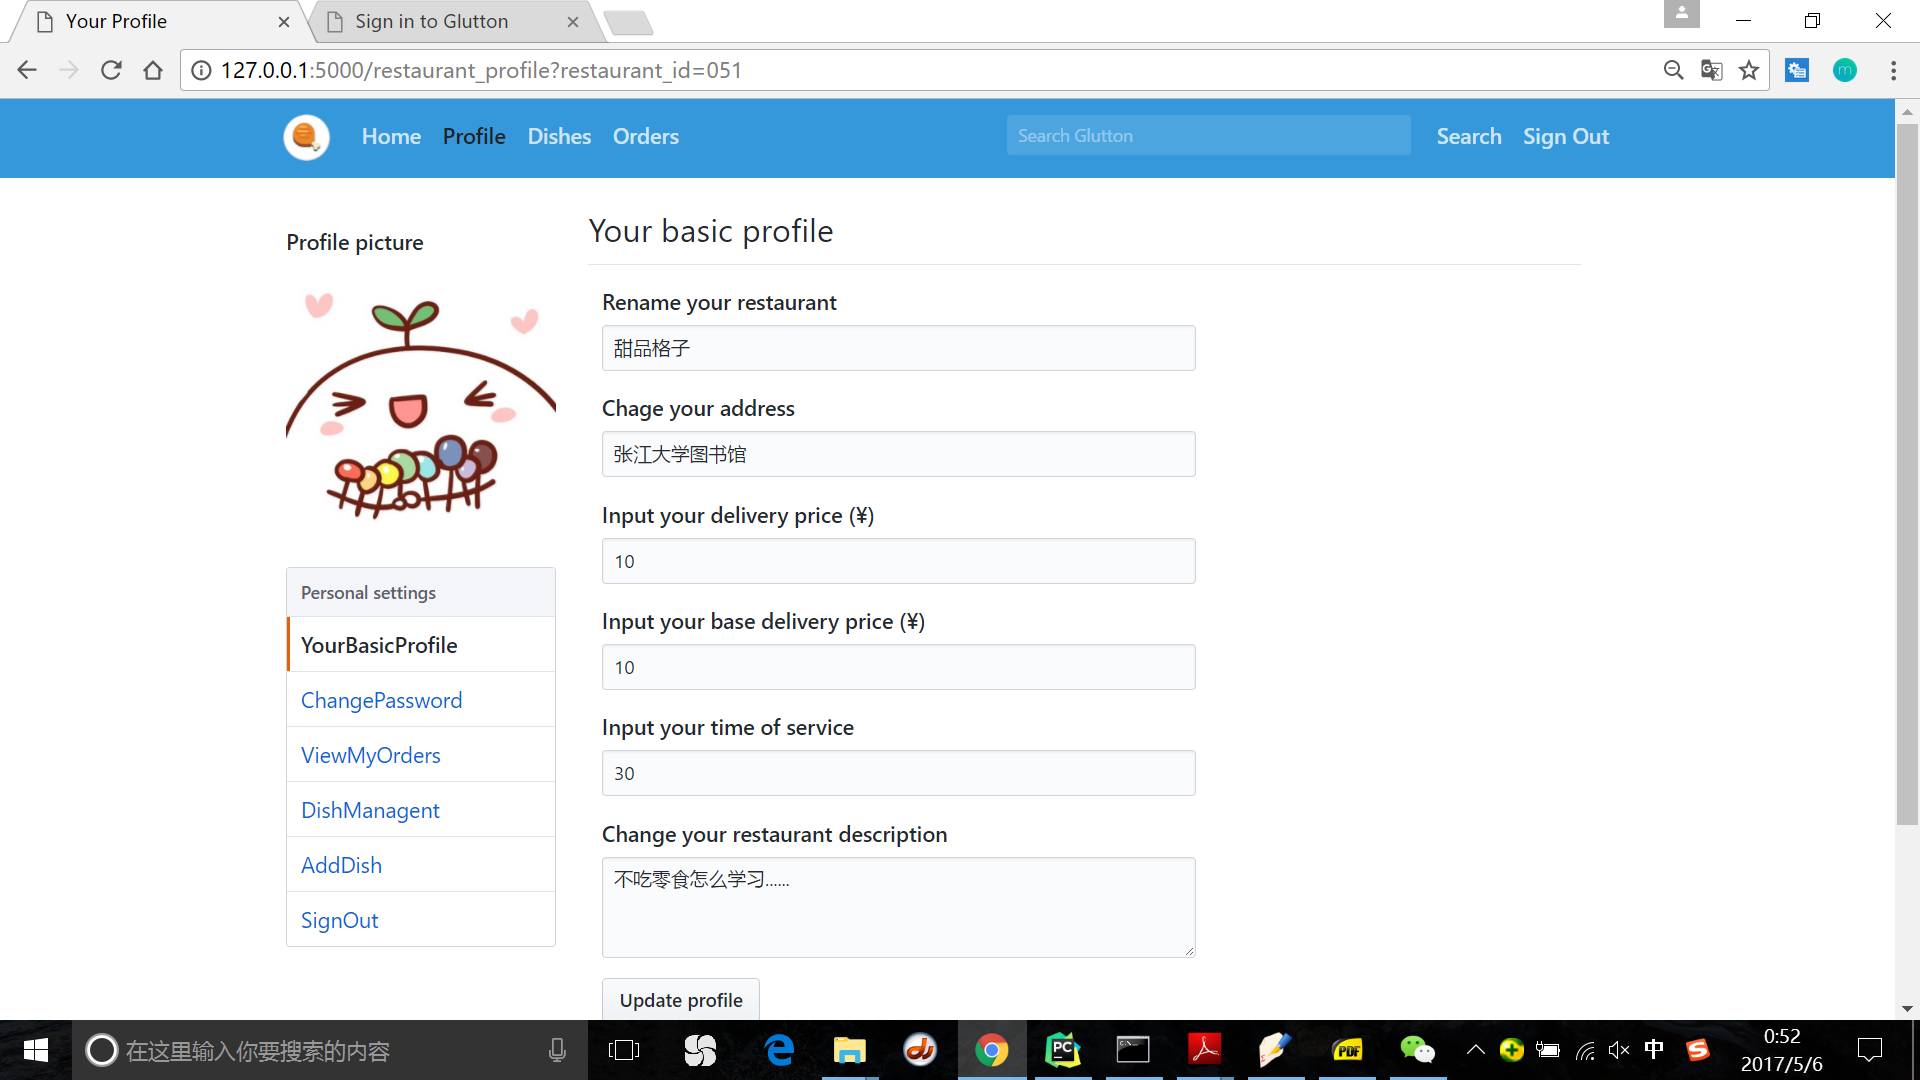
\includegraphics[width=3.2in]{re-profile.jpg}
     \caption{\small{商家更改信息}}\label{fig:dummy}
   \end{minipage}
   \begin{minipage}[t]{0.5\linewidth}
    \centering
     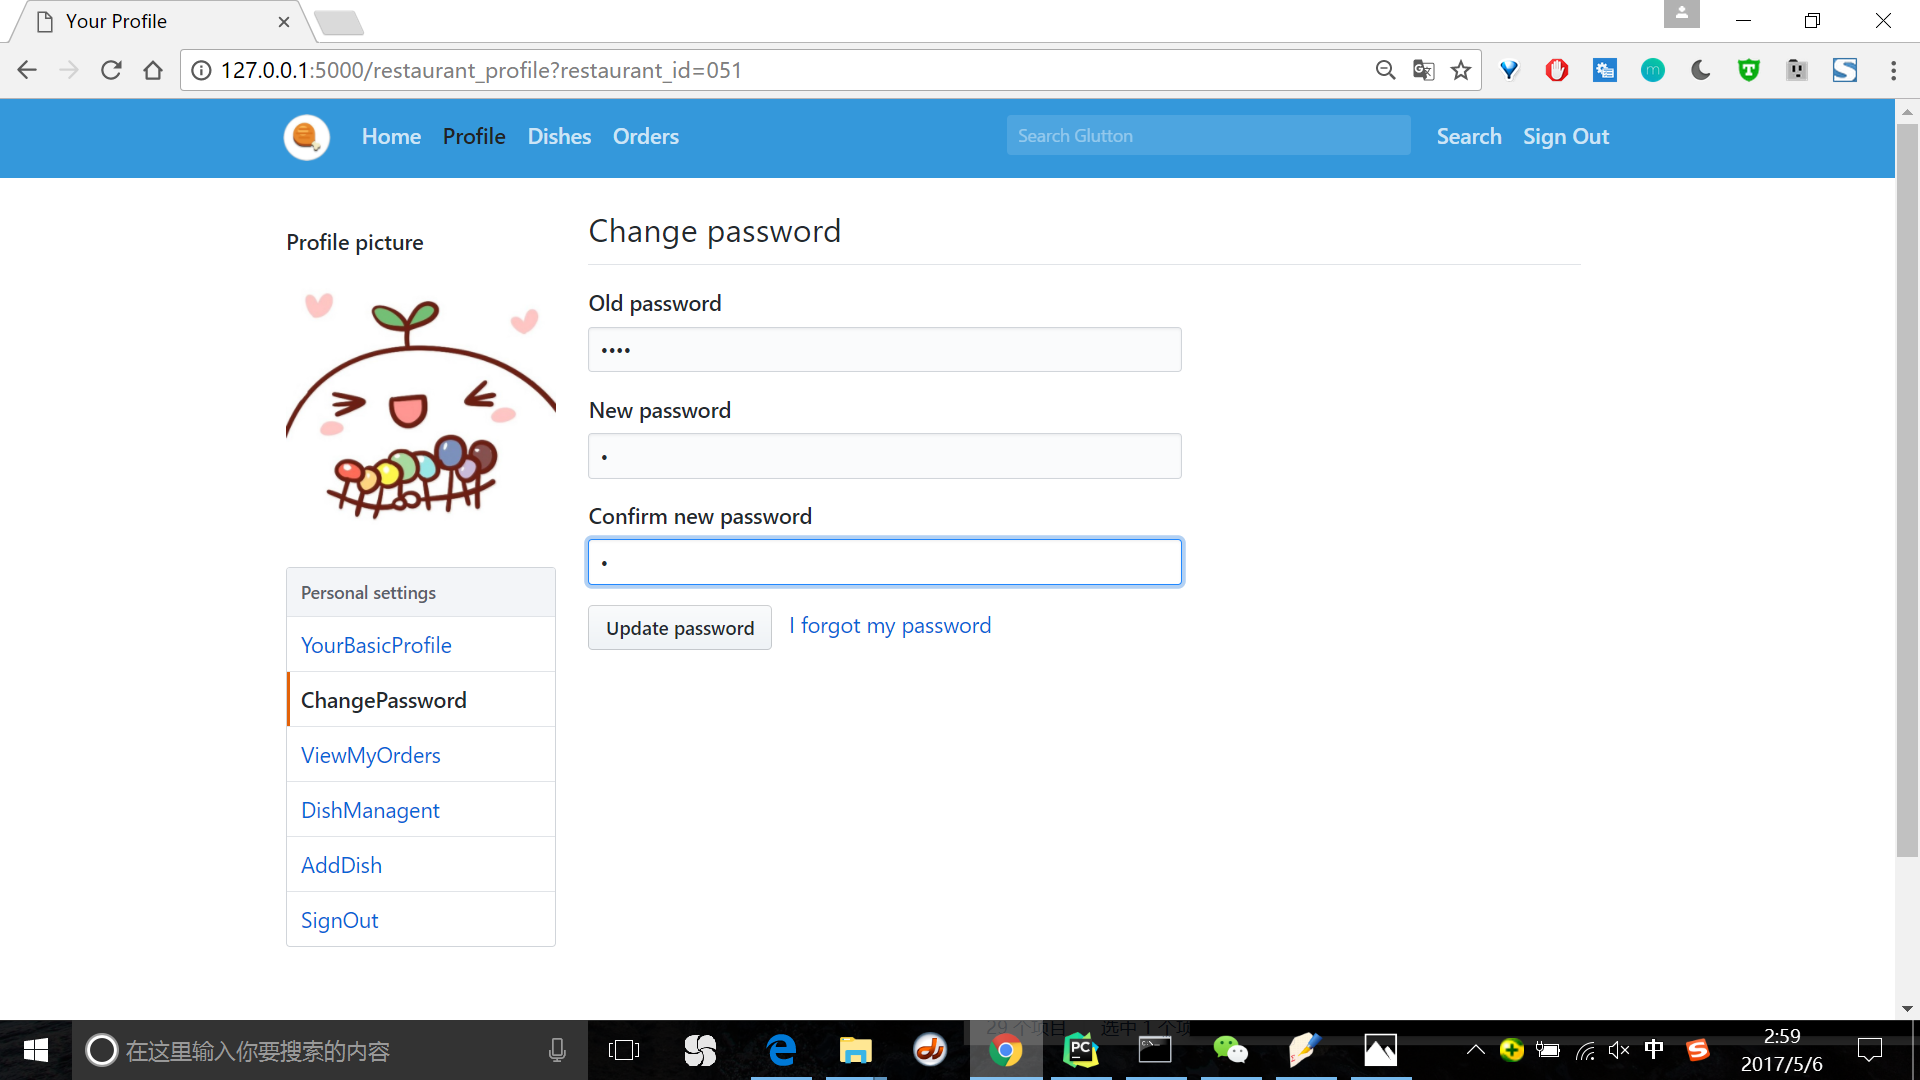
\includegraphics[width=3.2in]{re-password.jpg}
      \caption{\small{商家更改密码}}\label{fig:dummy}
   \end{minipage}
   \end{figure}
  \item 增加菜品\\
  点击AddDish按钮可以添加菜品,需要填写菜品名和价格,菜品添加成功,系统提示载入成功。\\
  我们也可以点击左侧DishManagement,或导航栏的Dishes进入菜品管理页面,会显示已有的菜品,并可以执行编辑、增加、删除操作。
  \begin{figure}[H]
   \begin{minipage}[t]{0.5\linewidth}
    \centering
     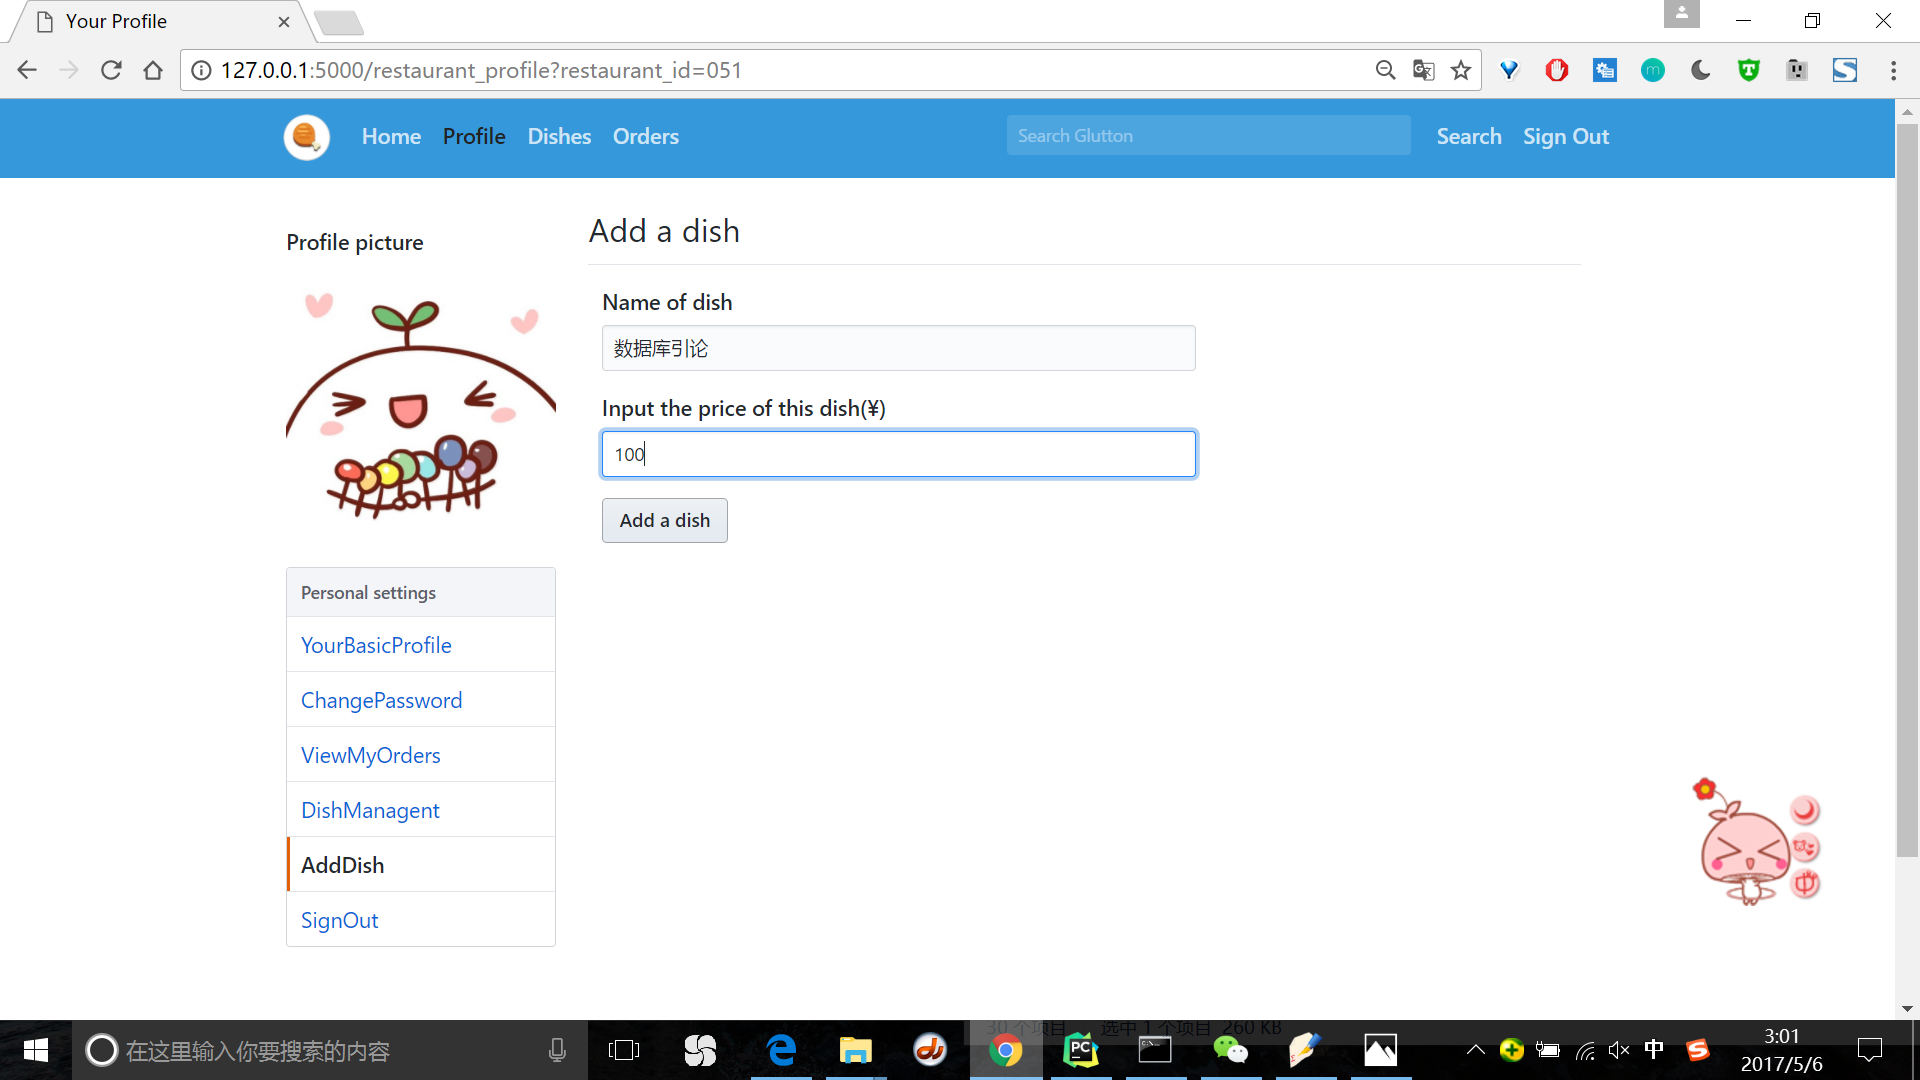
\includegraphics[width=3.2in]{re-add.jpg}
     \caption{\small{商家增加菜品}}\label{fig:dummy}
   \end{minipage}
   \begin{minipage}[t]{0.5\linewidth}
    \centering
     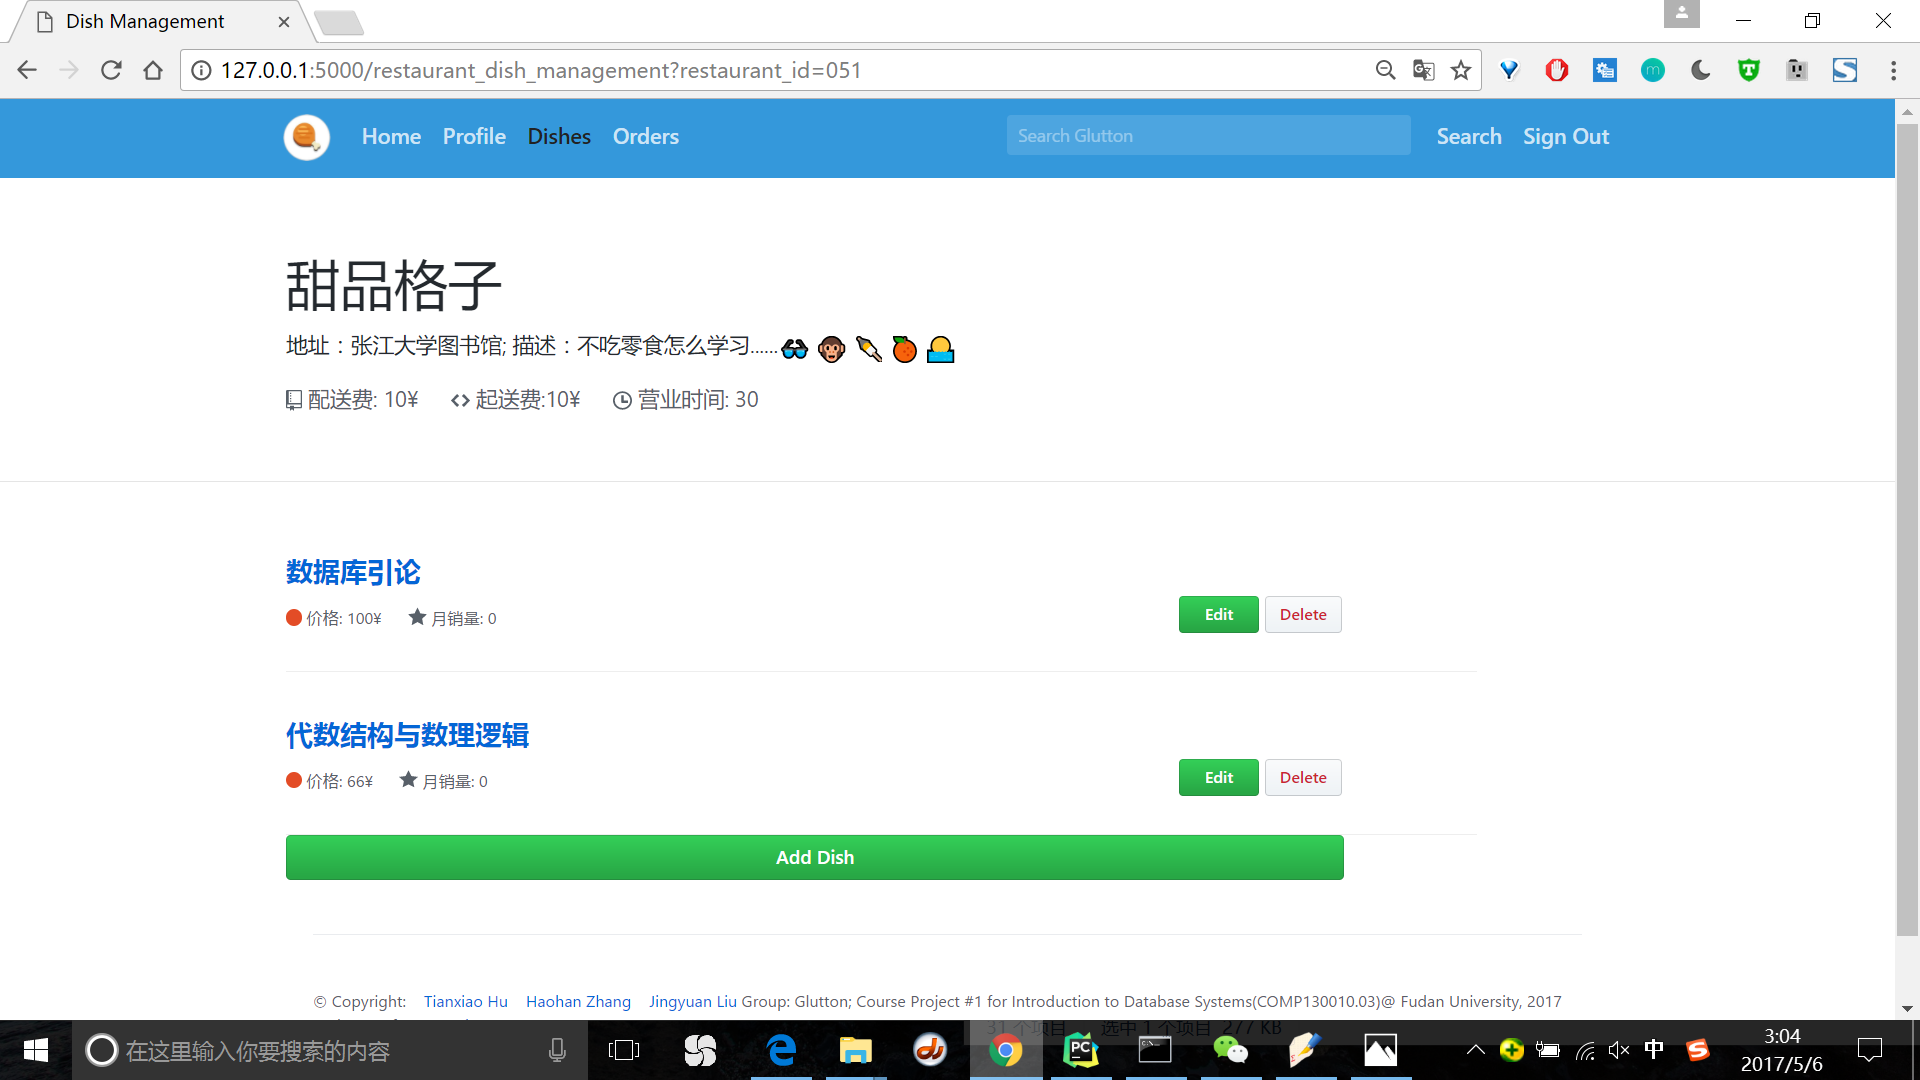
\includegraphics[width=3.2in]{re-dish.jpg}
      \caption{\small{商家查看菜品}}\label{fig:dummy}
   \end{minipage}
   \end{figure}
  \item 修改菜品\\
  在菜品管理页面中,点击Edit按钮,可以对菜品名,单价进行修改。
  \begin{figure}[H]
   \begin{minipage}[t]{0.5\linewidth}
    \centering
     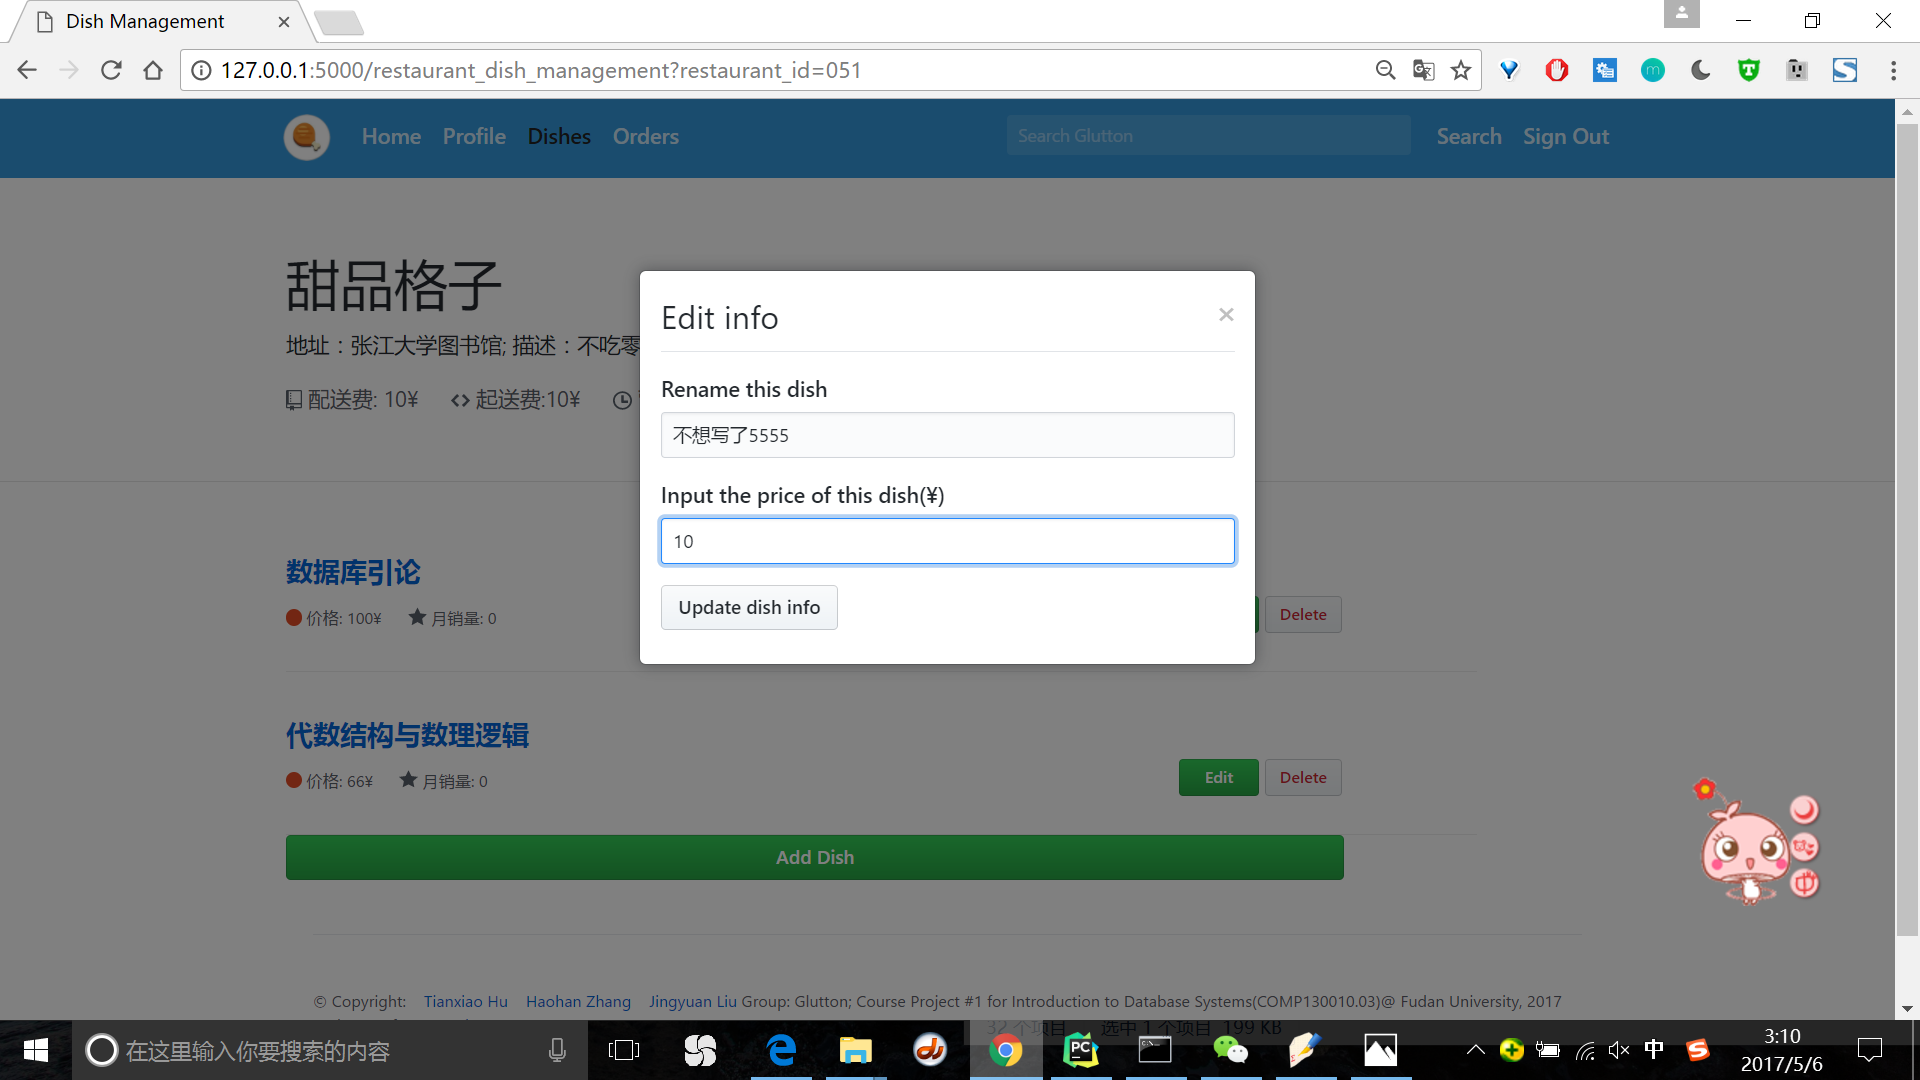
\includegraphics[width=3.2in]{re-update-dish1.jpg}
     \caption{\small{商家修改菜品信息}}\label{fig:dummy}
   \end{minipage}
   \begin{minipage}[t]{0.5\linewidth}
    \centering
     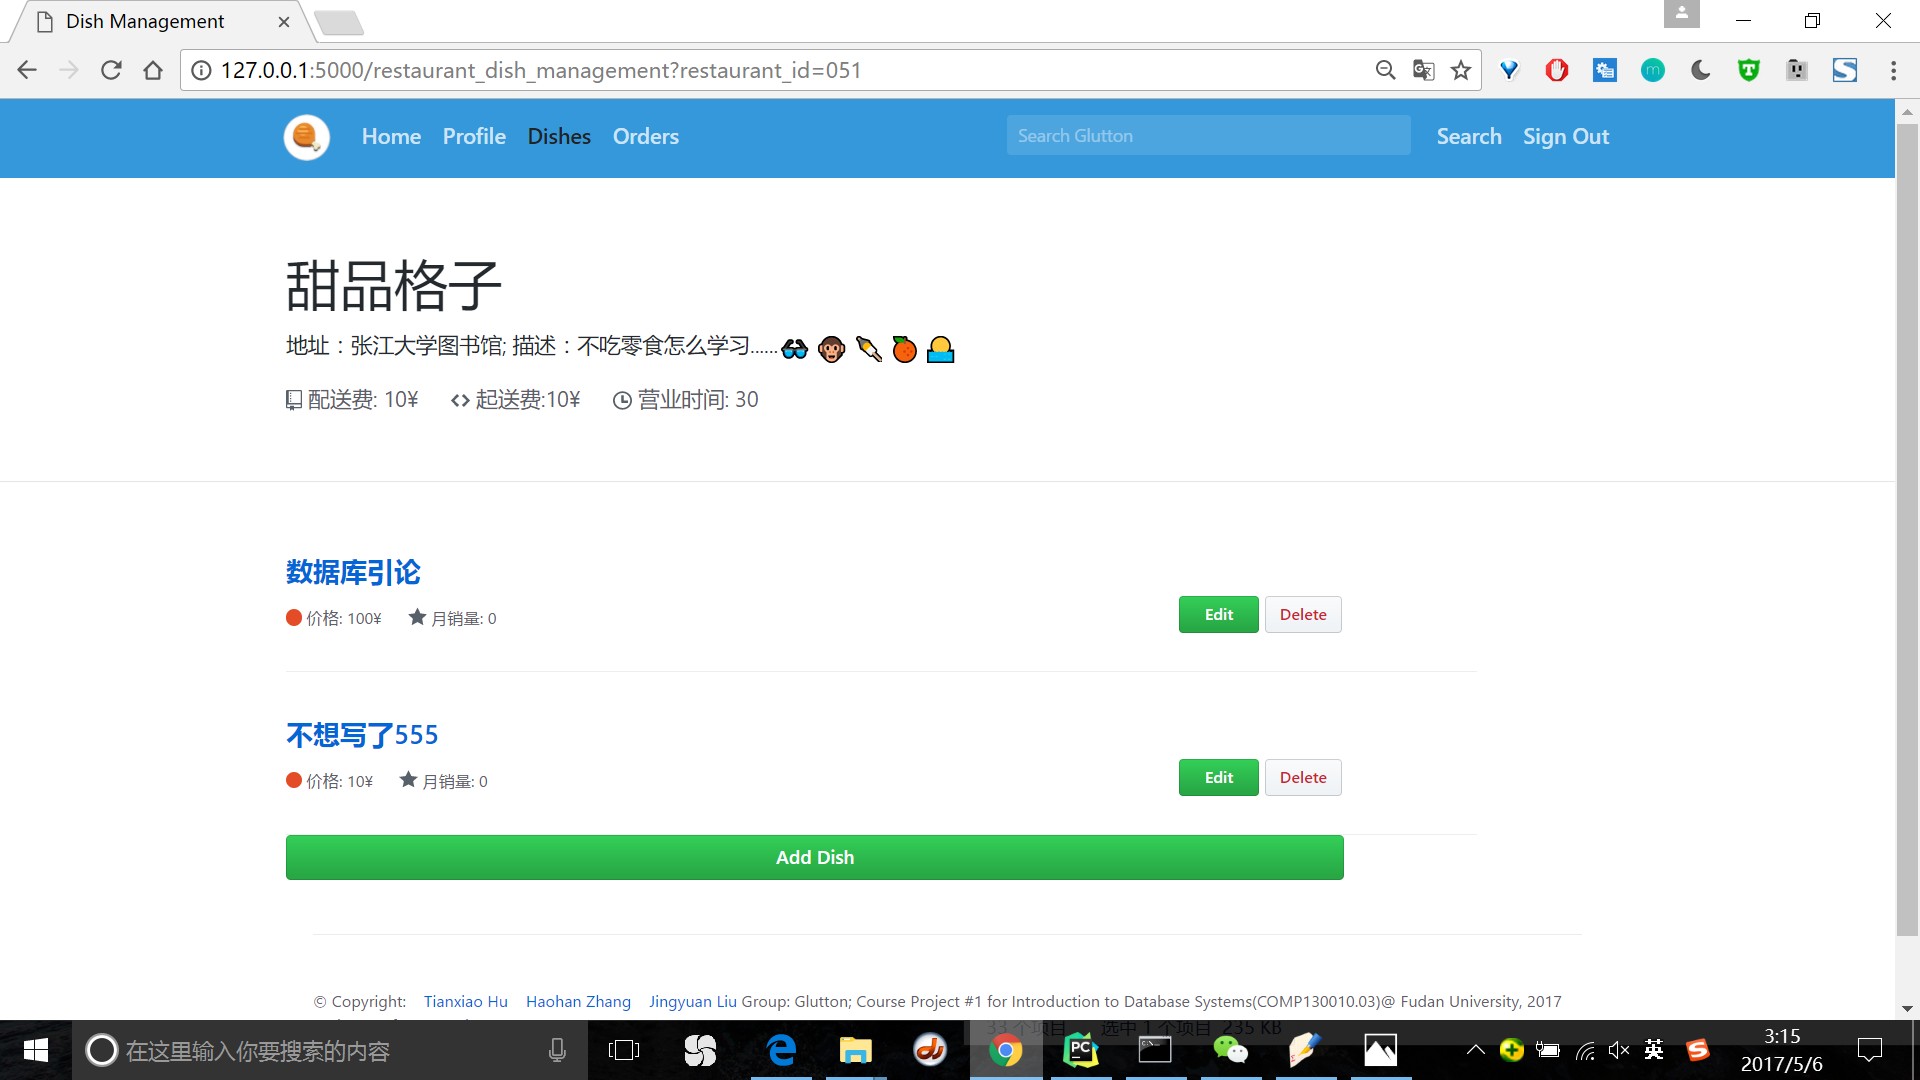
\includegraphics[width=3.2in]{re-update-dish2.jpg}
      \caption{\small{商家修改菜品后}}\label{fig:dummy}
   \end{minipage}
   \end{figure}
  \item 删除菜品\\
  在菜品管理页面中,点击Delete按钮,可以对菜品删除。系统会提示是否确定要删除该菜品,确定后,提示菜品删除成功,并跳转到菜品管理页面。
  \begin{figure}[H]
   \begin{minipage}[t]{0.5\linewidth}
    \centering
     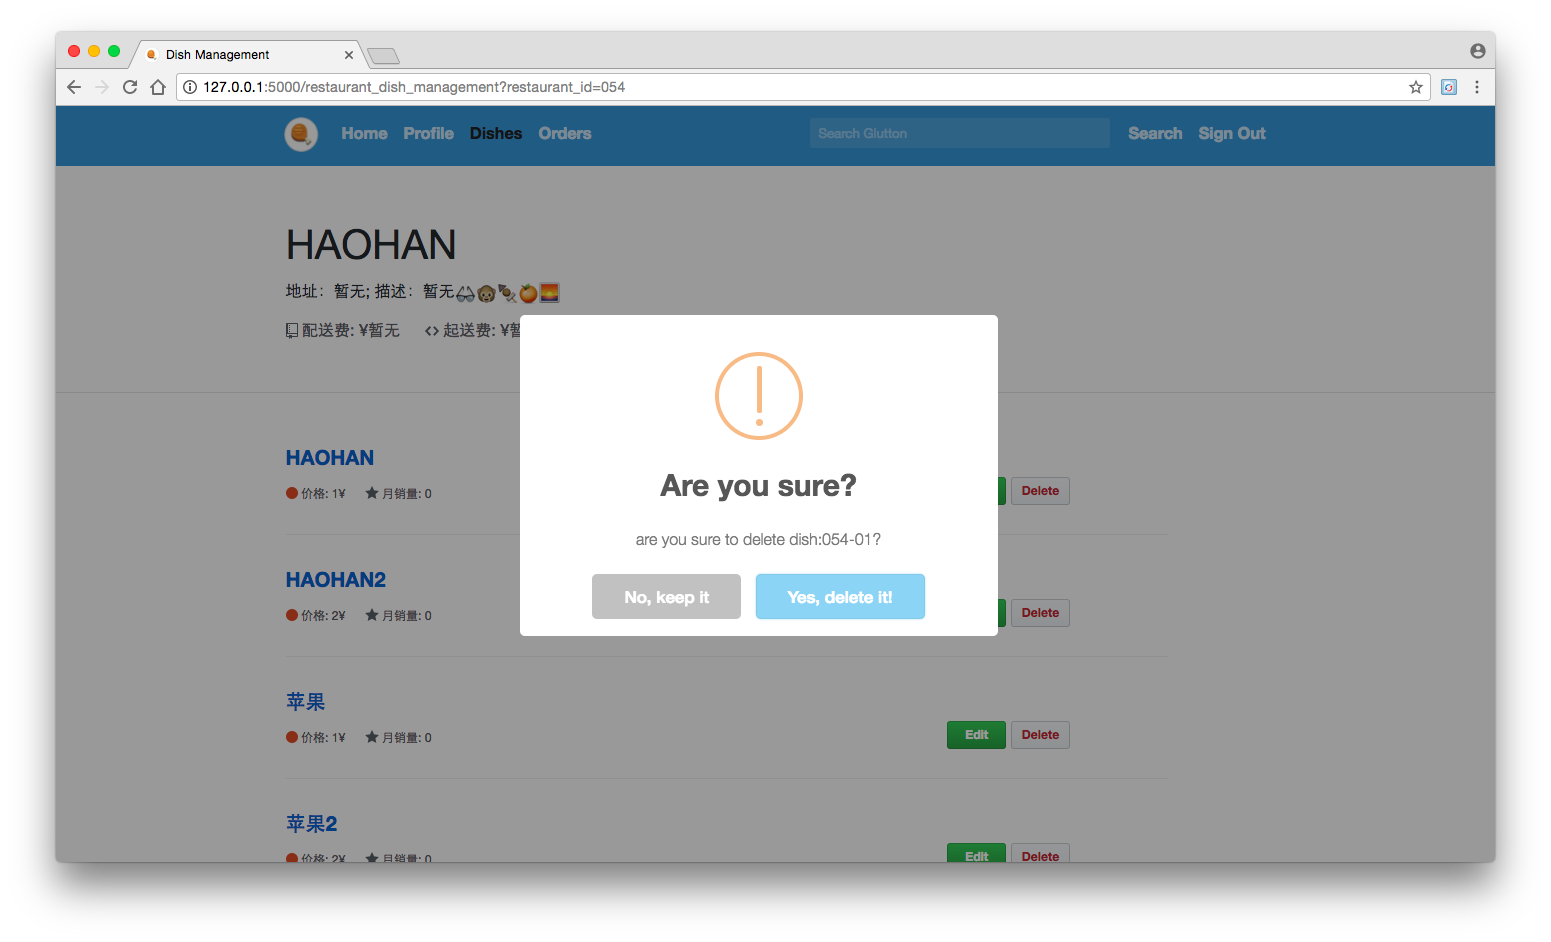
\includegraphics[width=3.2in]{re-delete-dish1.jpg}
     \caption{\small{商家删除菜品}}\label{fig:dummy}
   \end{minipage}
   \begin{minipage}[t]{0.5\linewidth}
    \centering
     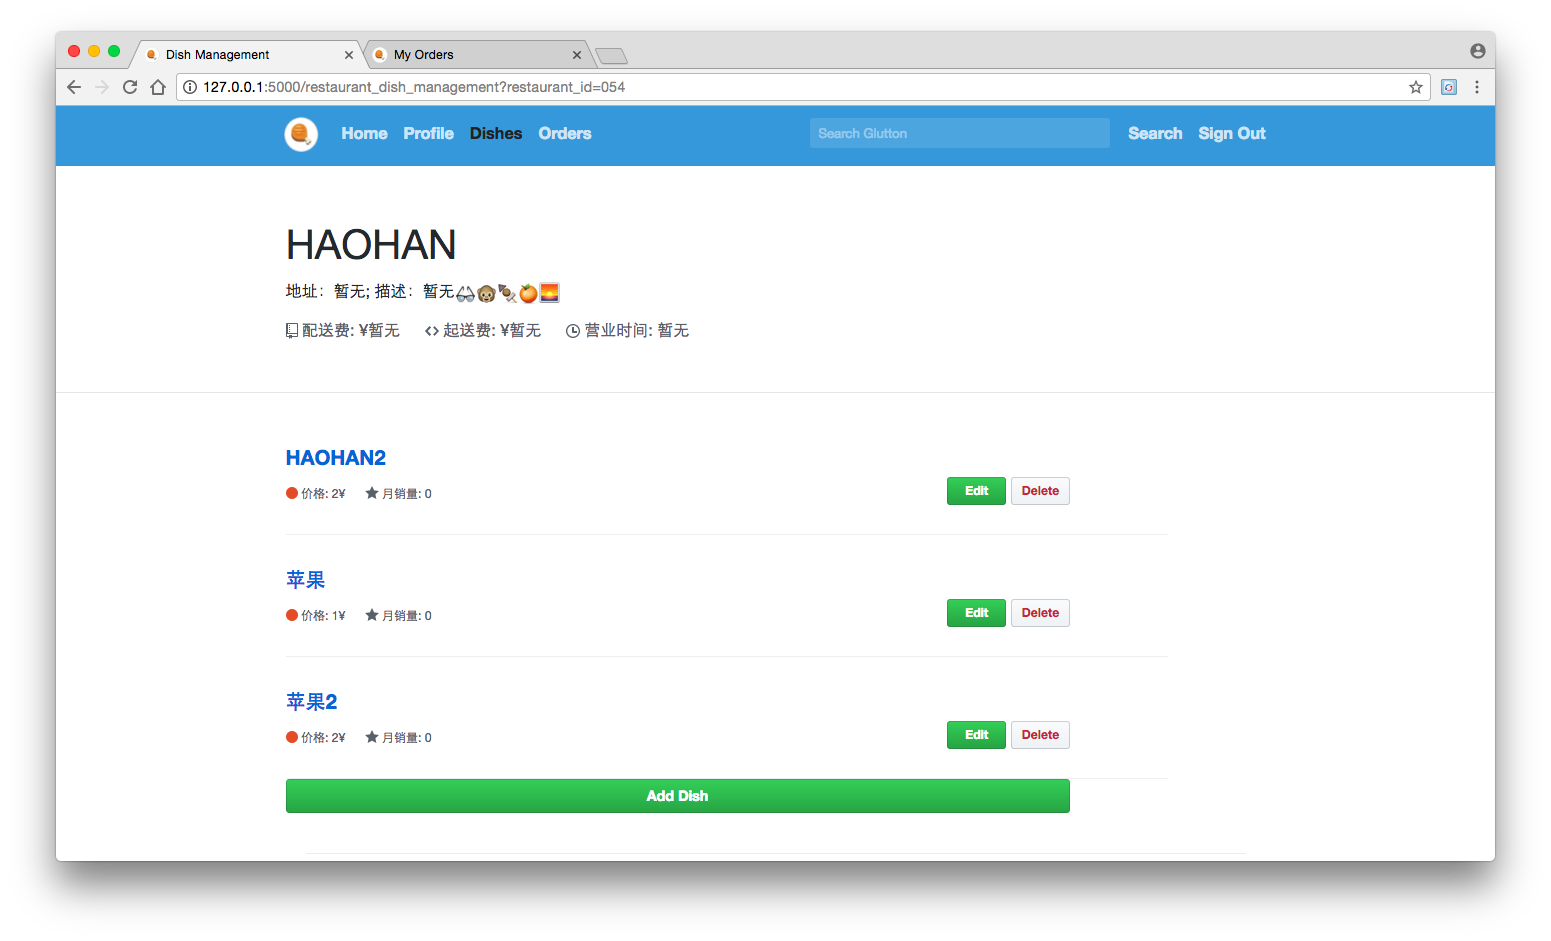
\includegraphics[width=3.2in]{re-delete-dish2.jpg}
      \caption{\small{商家删除菜品后}}\label{fig:dummy}
   \end{minipage}
   \end{figure}
  \item 查看商家订单历史\\
  新开的店铺订单信息为空,我们以用户身份登录,下单这家店铺的菜品,可以看到所有订单信息。\\
  我们还可以查看每个订单的评论。
  \begin{figure}[H]
   \begin{minipage}[t]{0.5\linewidth}
    \centering
     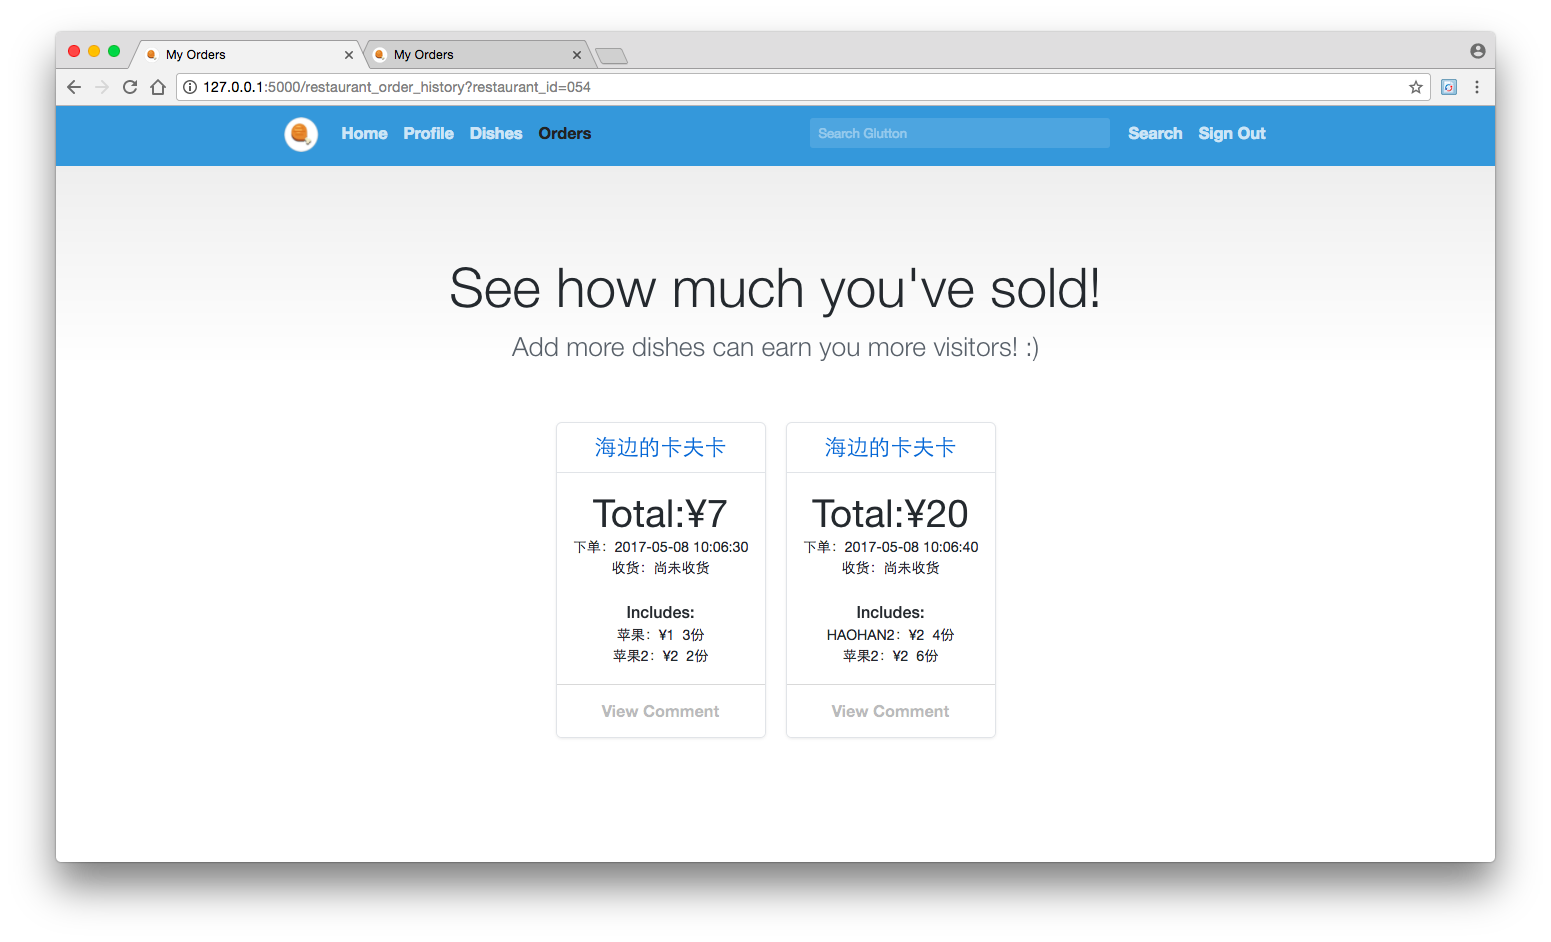
\includegraphics[width=3.2in]{re-order.jpg}
     \caption{\small{商家查看订单历史}}\label{fig:dummy}
   \end{minipage}
   \begin{minipage}[t]{0.5\linewidth}
    \centering
     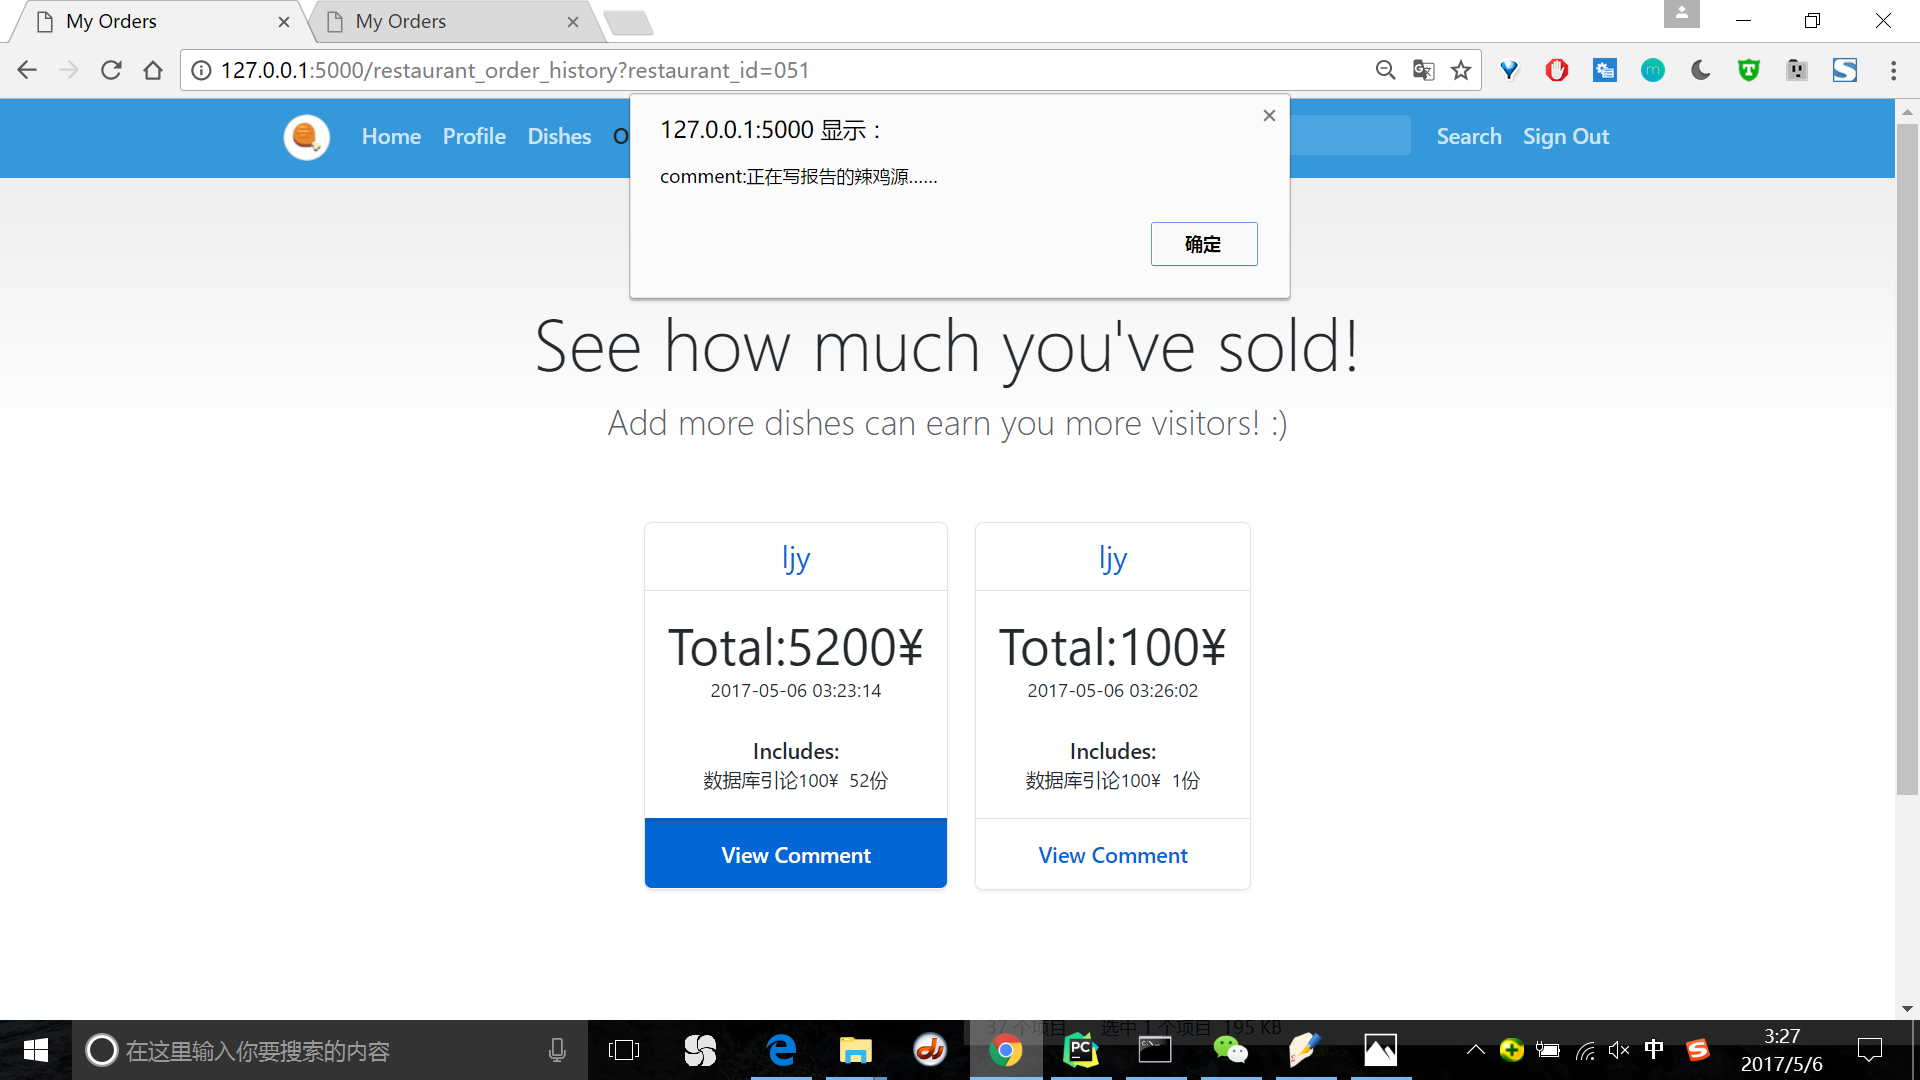
\includegraphics[width=3.2in]{re-order-comment.jpg}
      \caption{\small{商家查看订单评价}}\label{fig:dummy}
   \end{minipage}
   \end{figure} 
  \end{itemize}

\section{数据库简介}
 \begin{itemize}
 \item 数据源
  \par\setlength{\parindent}{1em}\normalsize 数据库Glutton所用数据来源于外卖平台”饿了么“网站,以复旦大学(张江校区)为中心,选取真实的商家信息作为数据源,保证了数据的真实性和有效性。
 \item 数据量
  \par\setlength{\parindent}{1em}\normalsize 数据选取以蔡伦路、科苑路、华佗路的商铺为主,涵盖50个商家。每个商家菜品若干,最多为17道菜,最少为4道菜,共393道菜,平均每个商家8(7.86)道菜。整个数据库包含443条商家及菜品记录。
 \item ER图
  \begin{figure}[H]
   \centering
     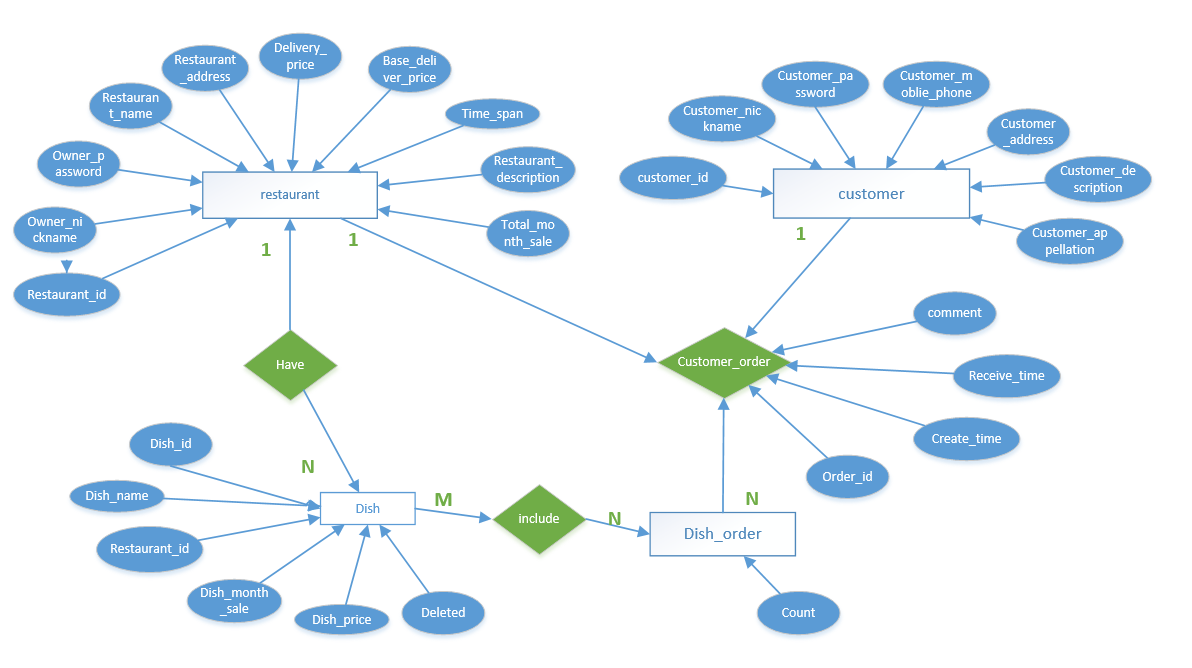
\includegraphics[width=7.00in]{ER.png}
     \caption{\small{数据库ER图}}\label{fig:dummy}
  \end{figure}

 \item 关系图
  \begin{figure}[H]
    \centering
     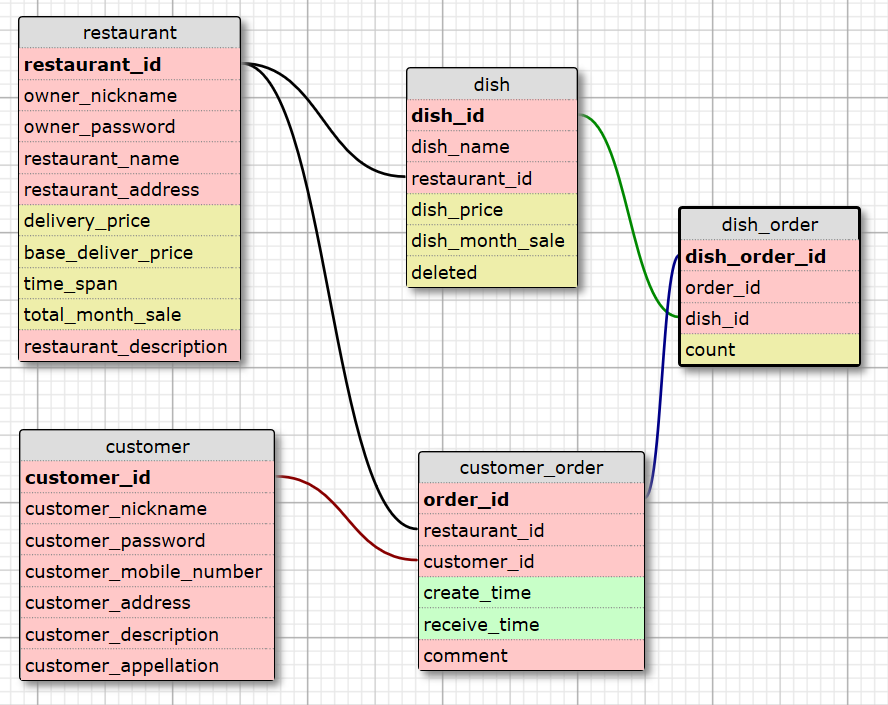
\includegraphics[width=7.00in]{tables.png}
     \caption{\small{数据库表格关系图}}\label{fig:dummy}
  \end{figure}

 \item 建表语句
 \par\setlength{\parindent}{1em}\normalsize 数据库Glutton共包含5张表:商家表、用户表、菜品表、用户订单表、菜品订单表。
 \begin{itemize}
 \item \textbf{商家表}信息包括:商家号、用户名、密码、商家名、商家地址、配送费、起送价、平均配送时间、营业时间、月销量、商家公告,主键为商家号。
      \begin{lstlisting}
   CREATE TABLE restaurant(
   restaurant_id CHAR(3) NOT NULL,
   owner_nickname CHAR(20) NOT NULL UNIQUE,
   owner_password CHAR(40) NOT NULL,
   restaurant_name CHAR(50) NOT NULL,
   restaurant_address CHAR(100),
   delivery_price DECIMAL(5,2),
   base_deliver_price DECIMAL(5,2),
   time_span SMALLINT,
   open_time  CHAR(20),
   total_month_sale INTEGER,
   restaurant_description CHAR(200),
   PRIMARY KEY(restaurant_id)
   );
\end{lstlisting}
 \item \textbf{用户表}信息包括:用户号、用户名、密码、手机号、收获地址、用户个人描述、用户称呼、用户口味偏好,主键为用户号,其中用户手机号应该是唯一的,加UNIQUE 区分。
      \begin{lstlisting}
   CREATE TABLE customer(
   customer_id CHAR(3) NOT NULL,
   customer_nickname CHAR(20) NOT NULL,
   customer_password CHAR(40) NOT NULL,
   customer_mobile_number CHAR(20) UNIQUE,
   customer_address CHAR(100),
   customer_description CHAR(100),
   customer_appellation CHAR(20),
   customer_avatar CHAR(20) NOT NULL,
   PRIMARY KEY(customer_id)
   );
      \end{lstlisting}
 \item \textbf{菜品表}信息包括:菜品号、菜品名、所属商家号、菜品价格、菜品月销量,主键为菜品号,外键为所属商家号,即可将菜品与商家联系起来。其中,商家删除菜品后,不能影响用户历史订单对这个菜品显示,所以加deleted属性。当商家删除菜品后,deleted为true,该菜品不在商家中显示,而用户历史订单中仍然可以查询到。
     \begin{lstlisting}
   CREATE TABLE dish(
   dish_id CHAR(6) NOT NULL,
   dish_name CHAR(30) NOT NULL,
   restaurant_id CHAR(3) NOT NULL,
   dish_price DECIMAL(5,2) NOT NULL,
   dish_month_sale SMALLINT,
   deleted BOOL,
   PRIMARY KEY(dish_id),
   FOREIGN KEY(restaurant_id)REFERENCES restaurant(restaurant_id)
   );
      \end{lstlisting}
 \item \textbf{用户订单表}信息包括:商家号、用户号、用户订单号、创建时间、收货时间、评论,主键为用户订单号,外键商家号、用户号分别关联商家表和用户表。
     \begin{lstlisting}
   CREATE TABLE customer_order(
   restaurant_id CHAR(3) NOT NULL,
   customer_id CHAR(3) NOT NULL,
   order_id CHAR(3) NOT NULL,
   create_time DATETIME NOT NULL,
   receive_time DATETIME,
   comment CHAR(100),
   PRIMARY KEY(order_id),
   FOREIGN KEY(restaurant_id)REFERENCES restaurant(restaurant_id),
   FOREIGN KEY(customer_id)REFERENCES customer(customer_id)
   );
      \end{lstlisting}
 \item \textbf{菜品订单表}信息包括:菜品订单号、用户订单号、菜品号、菜品数量,主键为菜品订单号,外键用户订单号、菜品号分别关联用户订单表和菜品表。这种设计使一个订单可以表示多个菜品,并减少了数据冗余。
     \begin{lstlisting}
   CREATE TABLE dish_order(
   dish_order_id CHAR(4) NOT NULL,
   order_id CHAR(4) NOT NULL,
   dish_id CHAR(6) NOT NULL,
   count SMALLINT NOT NULL ,
   PRIMARY KEY(dish_order_id),
   FOREIGN KEY(order_id)REFERENCES customer_order(order_id) ON DELETE CASCADE,
   FOREIGN KEY(dish_id)REFERENCES dish(dish_id)
   );
      \end{lstlisting}
 \end{itemize}

 \item 插入语句
 \par\setlength{\parindent}{1em}\normalsize 利用INSERT语句向数据库中插入商家、菜品、用户、订单信息。
  \begin{itemize}
   \item 建立数据库时的数据插入
    \begin{lstlisting}
   //插入商家信息
   INSERT INTO restaurant VALUES
   ('001','restaurant1','password','学城粥铺','上海市浦东新区张江镇华佗路572 号',2,0,45,'09:00-23:00',743,
   '需要米饭的亲们,可以在商品里面点哦,我们的炒菜是不配米饭的,除了商务套餐和盖浇饭以外,敬请谅解');
   //插入菜品信息
   INSERT INTO dish VALUES
   ('002-10','伴鸡伴虾堡','002',19,7);
    \end{lstlisting}
   \item 应用期间的数据插入
    \begin{lstlisting}
   //用户在创建账号时插入:用户ID,用户名,用户密码,用户手机号,用户口味偏好
   INSERT INTO customer VALUES
   ('%s', '%s', '%s', '%s', NULL, NULL, NULL, '1');
   //用户在创建订单时,插入用户订单信息:商家号、用户号、用户订单号、创建时间
   INSERT INTO customer_order VALUES
   ('%s', '%s', '%s', '%s', NULL, NULL);
   //用户在创建订单时,插入菜品订单信息:菜品订单号、用户订单号、菜品号、菜品数量
   INSERT INTO dish_order VALUES
   ('%s', '%s', '%s', '%d');
   //商家在新开一家店铺时,插入店铺信息:商家号、用户名、密码、商家名
   INSERT INTO restaurant VALUES
   ('%s', '%s', '%s', '%s', NULL, NULL, NULL, NULL, NULL, NULL, NULL);
   //……
    \end{lstlisting}
  \end{itemize}

 \item 查询语句
  \par\setlength{\parindent}{1em}\normalsize 利用SELECT语句查询商家、菜品、订单信息。
  \begin{itemize}
   \item 商家
    \par\setlength{\parindent}{1em}\normalsize 可以查看自己店铺的菜品和订单,并可以选择以一定的顺序(如菜品月销量,订单创建时间等)列表显示。
    \begin{lstlisting}

    \end{lstlisting}
   \item 用户
    \par\setlength{\parindent}{1em}\normalsize 用户可以查询某一店铺、菜品,按照某一顺序查看所有商家、菜品,查询自己的订单历史记录等,部分代码如下:
    \begin{lstlisting}
   //用户模糊查询某商家
   SELECT * FROM restaurant WHERE restaurant_name LIKE '%%%s%%';
   //用户模糊查询某道菜品
   SELECT dish_id, dish_name, dish.restaurant_id, dish_price, dish_month_sale,restaurant_name FROM dish, restaurant
   WHERE dish_name LIKE '%%%s%%'
   AND dish.restaurant_id = restaurant.restaurant_id AND NOT deleted;
   //用户按照最低起送价顺序查询商家
   SELECT * FROM restaurant
   WHERE restaurant_name LIKE '%%%s%%'
   ORDER BY base_deliver_price
   //用户按照最高月销量顺序查询商家
   SELECT * FROM restaurant
   WHERE restaurant_name LIKE '%%%s%%'
   ORDER BY total_month_sale DESC
   //用户按照最低价格顺序查询菜品
   SELECT dish_id, dish_name, dish.restaurant_id, dish_price, dish_month_sale,restaurant_name
   FROM dish, restaurant WHERE dish_name LIKE '%%%s%%' AND dish.restaurant_id = restaurant.restaurant_id AND NOT deleted
   ORDER BY dish_price
   //用户按照最高月销量顺序查询菜品
   SELECT dish_id, dish_name, dish.restaurant_id, dish_price, dish_month_sale, restaurant_name FROM dish, restaurant
   WHERE dish_name LIKE '%%%s%%' AND dish.restaurant_id = restaurant.restaurant_id AND NOT deleted
   ORDER BY dish_month_sale DESC
   //……
    \end{lstlisting}
  \end{itemize}

 \item 更改语句
  \par\setlength{\parindent}{1em}\normalsize 利用update语句修改商家、菜品、用户、订单等信息。
  \begin{itemize}
   \item 商家
   \begin{lstlisting}
   //商家修改店铺信息:商家名、商家地址、配送费、起送价,营业时间,店铺公告
   UPDATE restaurant SET restaurant_name = '%s', restaurant_address = '%s',
   delivery_price = '%s', base_deliver_price = '%s', open_time = '%s',
   restaurant_description = '%s' WHERE restaurant_id = '%s';
   //商家修改菜品信息:
   UPDATE dish SET dish_price = '%f', dish_name = '%s'  WHERE dish_id = '%s';
   \end{lstlisting}
   \item 用户
   \begin{lstlisting}
   //用户修改个人信息:用户名,用户地址,用户描述
   UPDATE customer SET customer_nickname = '%s', customer_address = '%s',
          customer_description = '%s', customer_appellation = '%s'
   WHERE customer_id = '%s'
   //用户修改密码
   UPDATE customer SET customer_password = '%s' WHERE customer_id = '%s';
   //用户修改个人口味偏好
   UPDATE customer SET customer_avatar = '%s' WHERE customer_id = '%s';
   \end{lstlisting}
  \end{itemize}

 \item 删除语句
   \par\setlength{\parindent}{1em}\normalsize 使用DELETE语句实现显式删除,UPDATE 语句结合菜品deleted属性实现隐式删除。
   \begin{itemize}
    \item 商家删除菜品
     \par\setlength{\parindent}{1em}\normalsize 采用隐式删除的方式,对于被删除的菜品,deleted属性被置为true,在商家列表中不再显示,且用户不能再查询到该菜品。但在用户历史订单中仍可以看到该菜品,这种设计更符合实际情况。
       \begin{lstlisting}
   UPDATE dish SET deleted = 1 WHERE dish_id = '%s'
       \end{lstlisting}
    \item 用户删除订单
     \par\setlength{\parindent}{1em}\normalsize 采用级联删除的方法,对于被删除的用户订单customer\_order,删除这一条元组的同时,在菜品订单dish\_order 表中同时删除以该订单为外键的菜品订单。
       \begin{lstlisting}

        \end{lstlisting}
   \end{itemize}


 \end{itemize}



\end{document}
